%% Ankur Sinha

%% packages %%
% support for coloured text
\usepackage{xcolor}
% moreland colour palette:
% https://github.com/Gnuplotting/gnuplot-palettes/blob/master/moreland.pal
% create: blue
\definecolor{moreland1}{HTML}{3b4cc0}
%visualise
\definecolor{moreland2}{HTML}{688aef}
%validate
\definecolor{moreland3}{HTML}{99baff}
%simulate
\definecolor{moreland4}{HTML}{c9d8ef}
%fit
\definecolor{moreland5}{HTML}{edd1c2}
%share
\definecolor{moreland6}{HTML}{f7a789}
%reuse
\definecolor{moreland7}{HTML}{e36a53}
% extra: red
\definecolor{moreland8}{HTML}{b40426}

% set 1 colour palette
% https://github.com/Gnuplotting/gnuplot-palettes/blob/master/set1.pal
% red
\definecolor{set11}{HTML}{E41A1C}
% blue
\definecolor{set12}{HTML}{377EB8}
% green
\definecolor{set13}{HTML}{4DAF4A}
% purple
\definecolor{set14}{HTML}{984EA3}
% orange
\definecolor{set15}{HTML}{FF7F00}
% yellow
\definecolor{set16}{HTML}{FFFF33}
% brown
\definecolor{set17}{HTML}{A65628}
% pink
\definecolor{set18}{HTML}{F781BF}

% IPA
\usepackage{tipa}
\usepackage[scale=2]{ccicons}
\usepackage{amssymb}
\usepackage{standalone}
\usepackage{tikz}
\usetikzlibrary{shapes.geometric,arrows,positioning,quotes,graphs,mindmap,decorations.pathmorphing,trees}
\usepackage{jneurosci}
\usepackage{subcaption}
\usepackage[T1]{fontenc}
\usepackage[utf8]{inputenc}
\usepackage[style=nature,backend=biber,autocite=footnote]{biblatex}
\addbibresource{/home/asinha/Documents/01_Readables/00_research_papers/bibliography/masterbib.bib}
\usepackage{roboto}
% for strike through
\usepackage[normalem]{ulem}
% links, urls, refs
\usepackage{hyperref}
\hypersetup{colorlinks,linkcolor=Green,urlcolor=set18}
% graphics
\usepackage{graphicx}
\graphicspath{{99_images/}}
% algorithm
\usepackage{algorithmic}
\usepackage{textcomp}
\usepackage{wrapfig}
\usepackage{textgreek}
\usepackage{euler}
\usepackage{tabularx}
\usepackage{booktabs}
\usepackage{minted}
\usepackage{csquotes}
% beamer theme
% use defaults for theme
\usetheme[progressbar=foot]{moloch}
% for page numbers
\setbeamertemplate{page number in head/foot}[appendixframenumber]
% for footnotes
% https://tex.stackexchange.com/questions/683533/beamer-theme-metropolis-does-not-allow-different-font-size-for-fullcite/683540#683540
\setbeamerfont{bibliography entry title}{size=}
\setbeamerfont{bibliography entry author}{size=}
\setbeamerfont{bibliography entry location}{size=}
\setbeamerfont{bibliography entry note}{size=}
%\usetheme[numbering=fraction,sectionpage=progressbar,subsectionpage=progressbar,progressbar=frametitle]{metropolis}
%\usefonttheme[onlymath]{serif}
\setbeamerfont{footnote}{size=\Tiny}
\setbeamerfont{caption}{size=\tiny}
\setbeamercolor{alerted text}{fg=Green}
\setbeamerfont{note page}{size=\small}
\setbeamercolor{alerted text}{fg=set15}
\setbeamercolor{progress bar}{fg=set18}
\setbeamercolor{title separator}{fg=set18}
\setbeamercolor{frametitle}{bg=moreland1}

\renewcommand{\figurename}{}

% Not needed in metropolis, but in general footnote citation fixes: https://tex.stackexchange.com/questions/44217/how-can-i-stop-footcite-from-hijacking-my-beamer-columns
% how to use multiple references to the same footnote: https://tex.stackexchange.com/questions/27763/beamer-multiple-references-to-the-same-footnote

% Disable footnoterule
\renewcommand{\footnoterule}{}
\renewcommand*{\bibfont}{\tiny}

%% title %%
\title{The NeuroML ecosystem for standardised multi-scale modelling in neuroscience}
\author[Ankur Sinha]{Ankur Sinha\\Silver Lab\\Department of Neuroscience, Physiology, \& Pharmacology\\University College London}
\date{2024-02-26}

%% document begins %%
\begin{document}


% title frame %%
\begin{frame}
  \titlepage{}
\end{frame}
%% Three slides for 5 minutes seems good
%% So, 30 slides at most for 50 minutes

% Why is biophysically detailed modelling important?
% Why are standards necessary?
%\section{Biophysically detailed models and standards}
\begin{frame}[c]
  \frametitle{An understanding of the brain}
  \begin{columns}
    \begin{column}{0.5\textwidth}
      \begin{figure}[h]
        \centering
        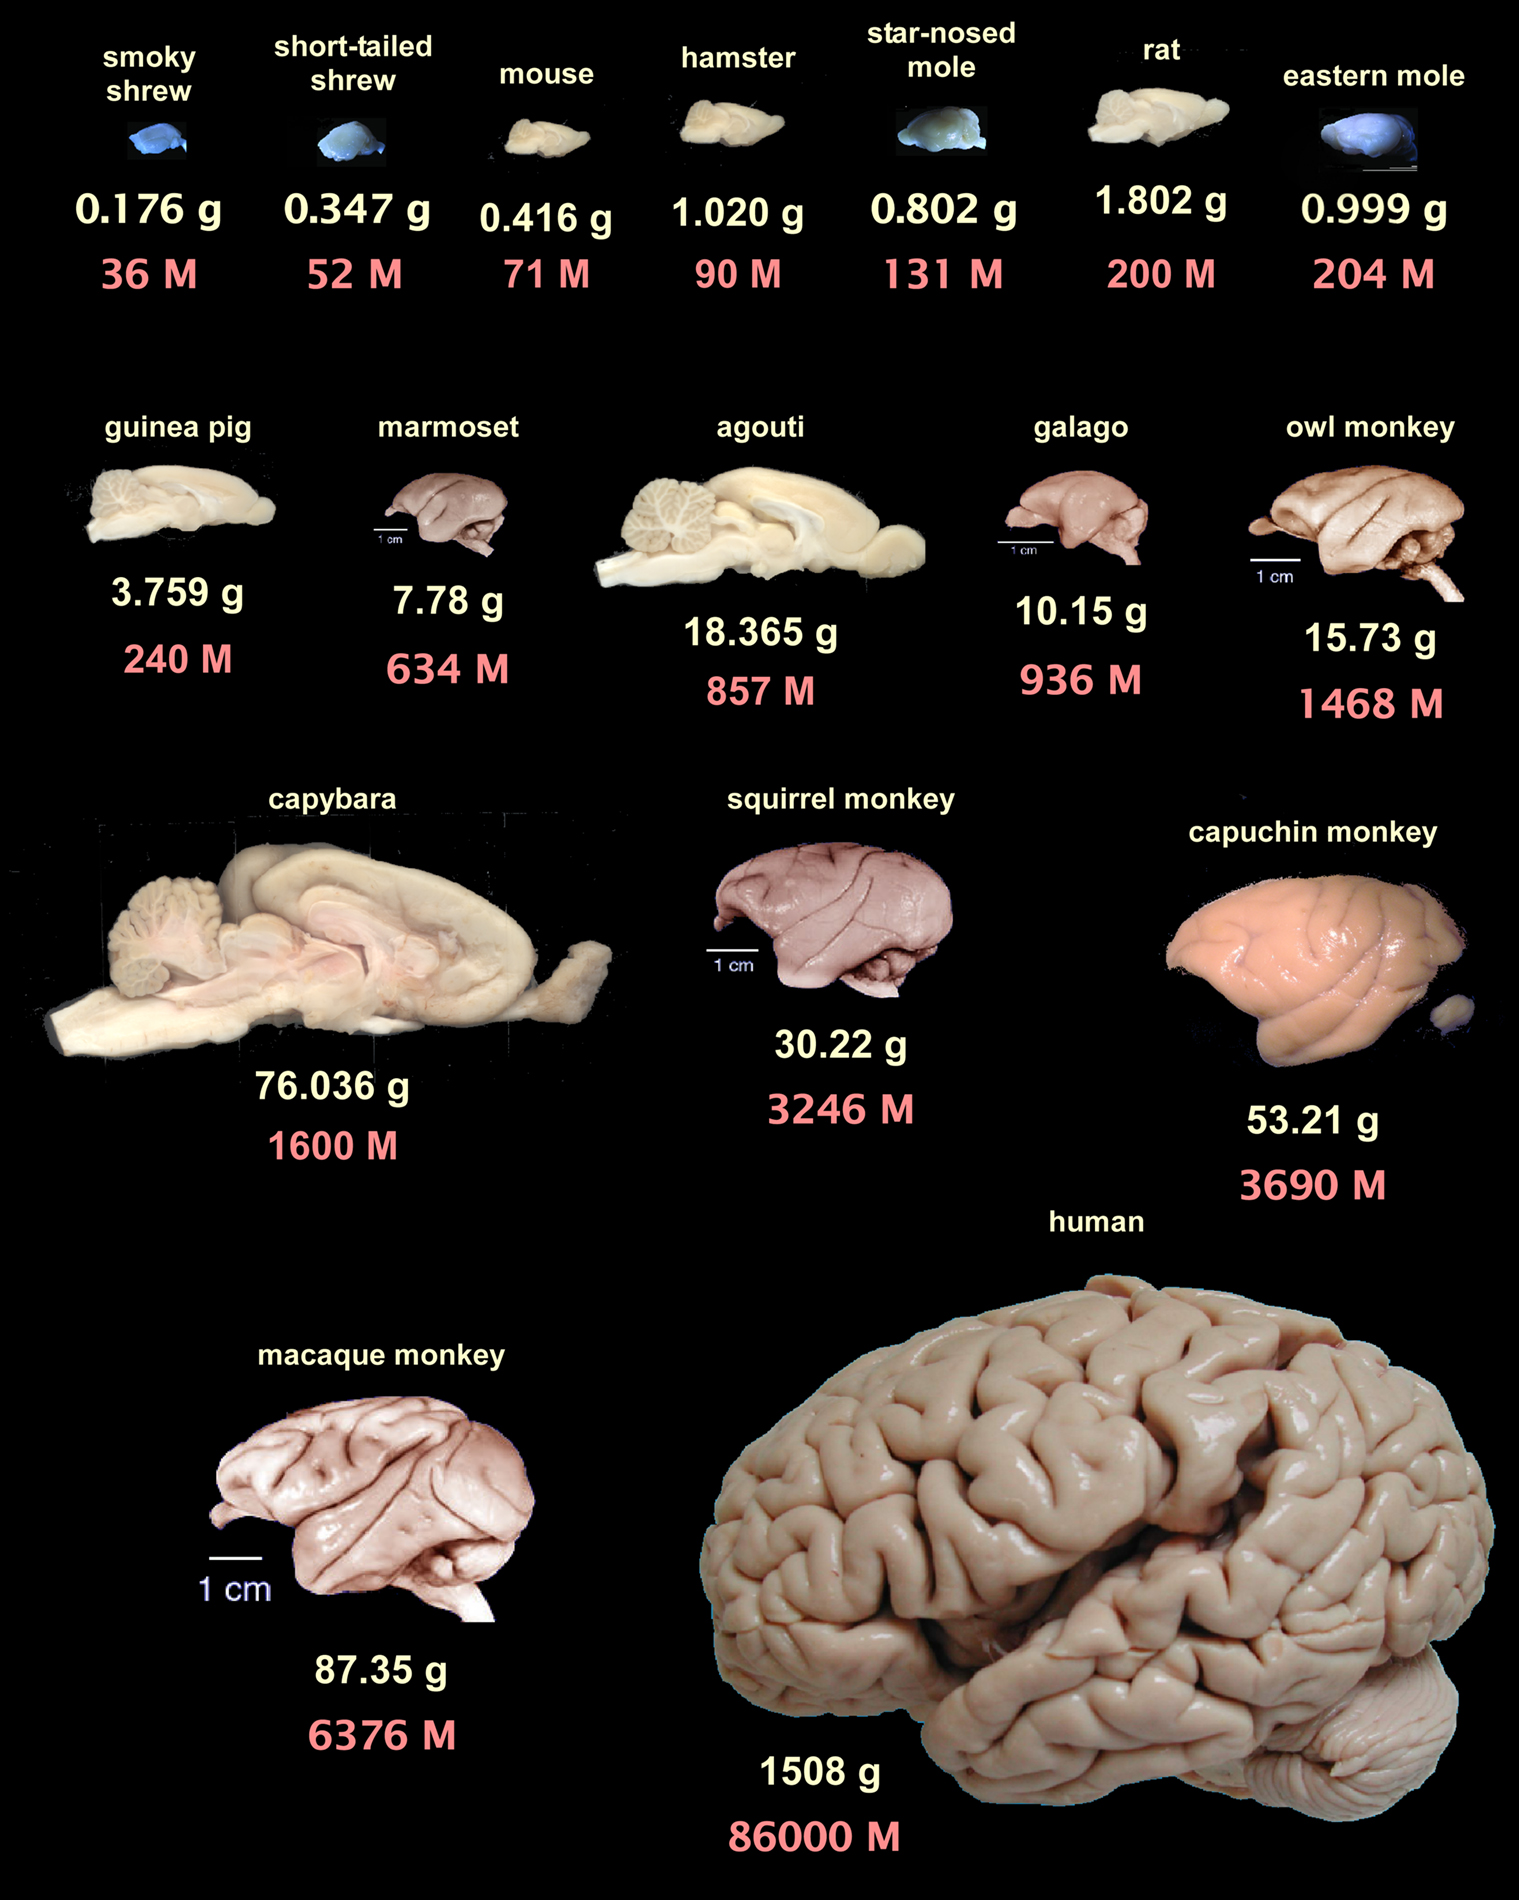
\includegraphics[width=\textwidth]{99_images/brain-sizes.jpg}
      \end{figure}
    \end{column}
    \begin{column}{0.5\textwidth}
      \begin{itemize}
        \only<1>{%
          \item<1> \alert{\textasciitilde 86B} neurons
          \item<1> \alert{\textasciitilde 100T} synapses
          \item<1> also \alert{\textasciitilde 85B} glia
        }
        \only<2>{%
          \item<2> specialised \alert{circuits}
          \item<2> different \alert{neuronal} types
          \item<2> \alert{synaptic} connections
          \item<2> complex \alert{sub-cellular} processes
        }
      \end{itemize}
    \end{column}
  \end{columns}
  \note[item]{We want to understand how the brain does things}
  \note[item]{This is important, not only for clinical applications---that is treatment of various brain disorders---but also because we want to understand the various algorithms that allow the brain to process such large amounts of information and react to the environment.}
  \note[item]{Now, to give you an idea of the size of the challenge: the most recent estimate puts the number of neurons in the human brain at 86B.}
  \note[item]{These are connected to each other with 100T synapses}
  \note[item]{Recently, we've also started to understand, rather realise, the importance of support cells---the glia---85B of them.}
  \vspace{0.2cm}
  \footnotetext[1]{{\tiny{\fullcite{HerculanoHouzel2009}}}}
  \footnotetext[1]{{\tiny{\fullcite{Bartheld2016}}}}
\end{frame}
\begin{frame}[c]
  \frametitle{Models complement experimental neuroscience}
  Models are fully \alert{observable}, \alert{controllable}.
  \pause{}
  \begin{itemize}
      \pause{}
    \item Combine individual experimental results into \alert{unified theories}
    \item Explore \alert{generalisability} of experimental results over wider range of conditions
    \item \alert{Generate} new experimentally testable, physically plausible hypotheses: \alert{dictate experiment design}
  \end{itemize}
  \note[item]{Now, experiments of course, provide us with direct evidence about the brain.}
  \note[item]{fMRI, EEG, to voltage and calcium imaging, patch clamp recordings}
  \note[item]{Now: large scale brain observatories}
  \note[item]{Models/theory are necessary for:}
  \note[item]{combining independent experimental results into unified theories}
  \note[item]{exploring these complex systems across wider range of conditions}
  \note[item]{generating new testable hypotheses}
\end{frame}
\begin{frame}[c]
  \frametitle{Models: different scales}
  \pause{}
  \begin{columns}
    \begin{column}{0.5\textwidth}
      \begin{figure}[h]
        \centering
        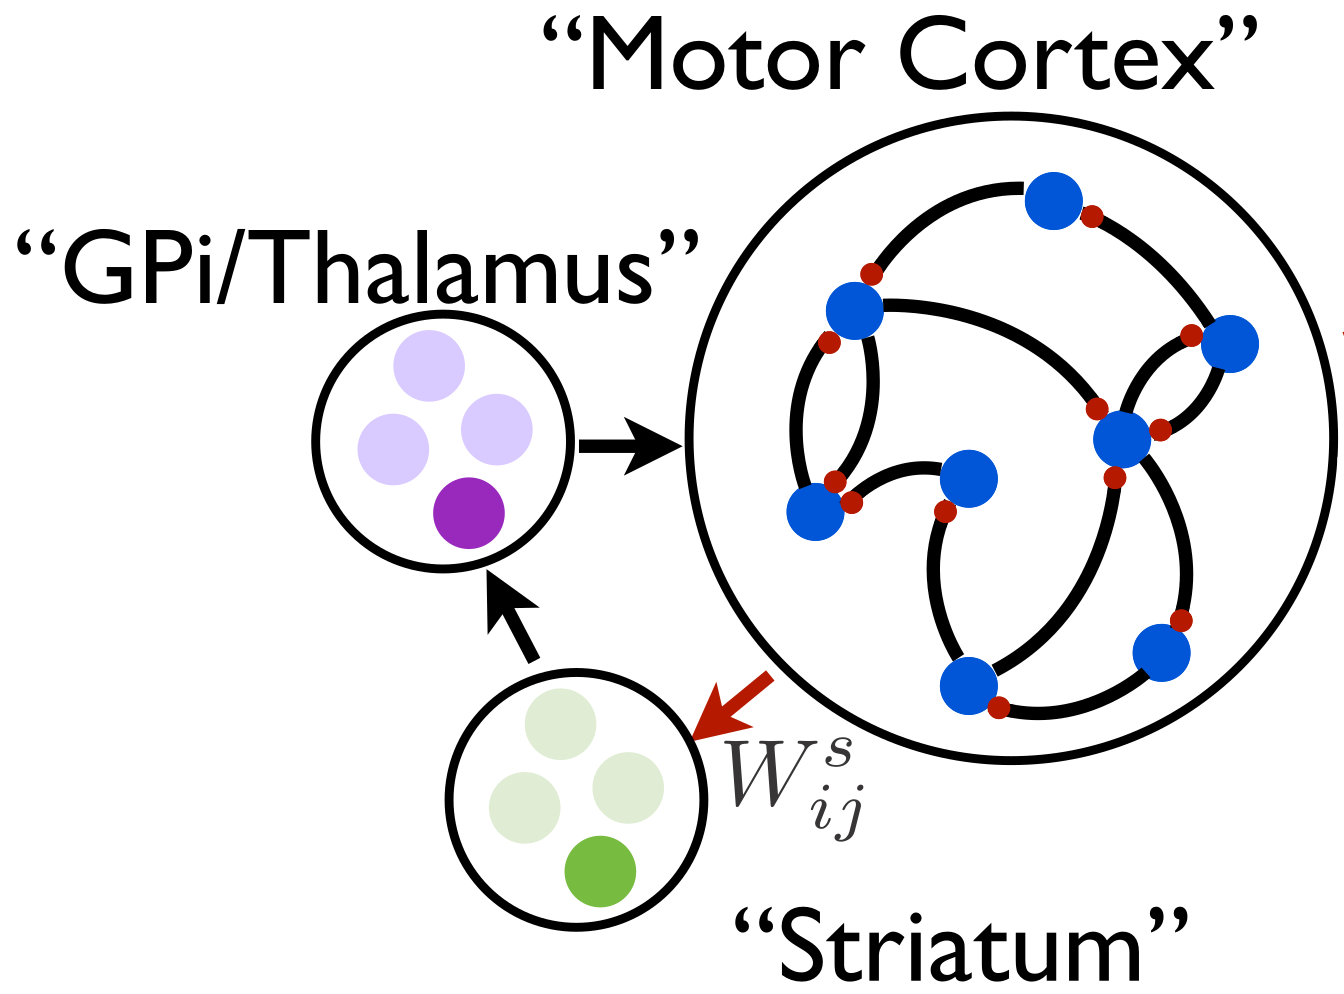
\includegraphics[width=0.8\textwidth]{99_images/Murray2019-4b}\\\vspace{0.2cm}
        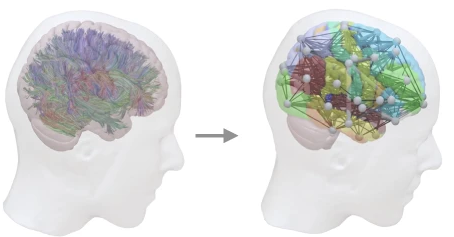
\includegraphics[width=0.9\textwidth]{99_images/TVB}\\
      \end{figure}%
    \end{column}
    \uncover<3>{%
    \begin{column}{0.5\textwidth}
      \begin{figure}[h]
        \centering
        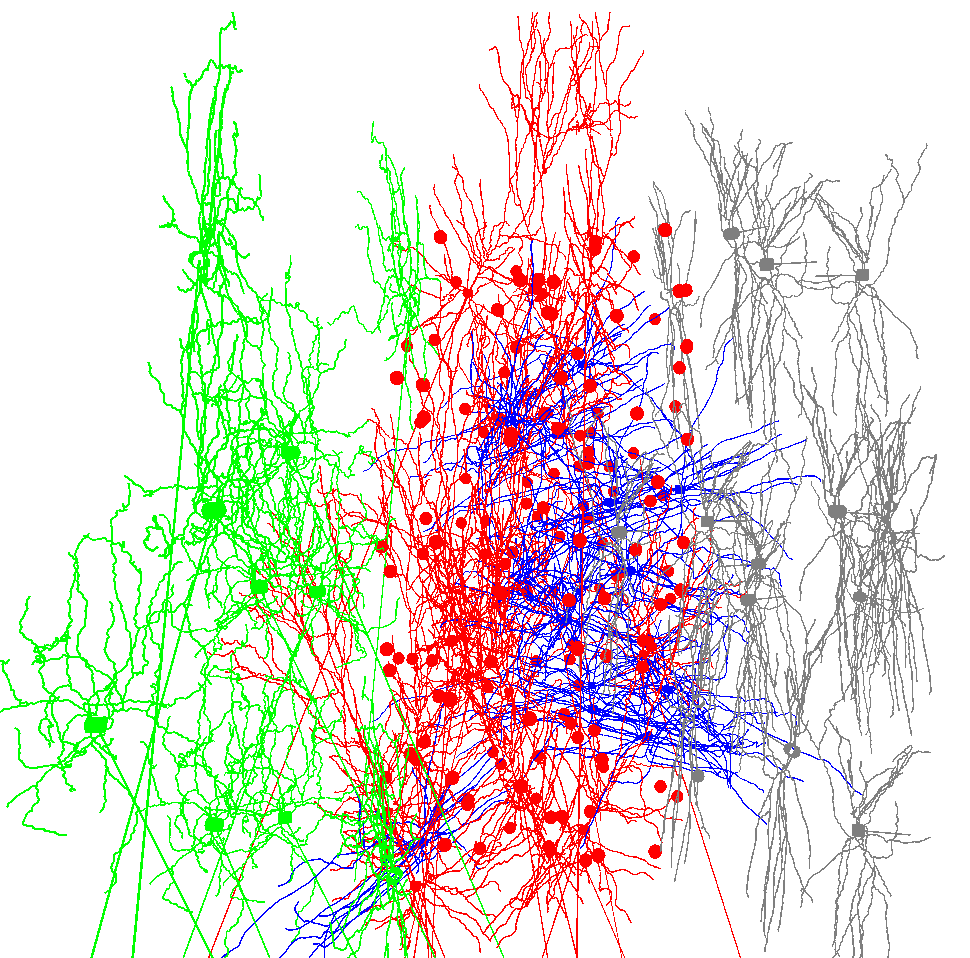
\includegraphics[width=0.65\textwidth]{99_images/20231004-HL23Net}\vspace{0.2cm}
        \includegraphics[width=0.7\textwidth]{99_images/Maeki2020}
      \end{figure}%
    \end{column}}
  \end{columns}
  \note[item]{RNNs are appropriate for lots of projects, for example.}
  \note[item]{So are whole brain neural mass models.}
  \note[item]{But, to really understand the underlying mechanisms that give rise to emergent behaviour, we must model the brain at biophysically detailed levels.}
  \only<2->{\footnotetext[1]{\fullcite{Murray2019}}}
  \only<2->{\footnotetext[1]{\fullcite{Schirner2023}}}
  \only<2->{\footnotetext[1]{\fullcite{Yao2022}}}
  \only<2->{\footnotetext[1]{\fullcite{MaekiMarttunen2020}}}
\end{frame}
\begin{frame}[c]
\frametitle{}
\begin{center}
\Large{A \alert{\emph{mechanistic}} understanding of the brain requires \alert{biophysically detailed} modelling}
\end{center}
\end{frame}
\begin{frame}[c]
  \frametitle{The model life cycle}
  \begin{figure}[h]
    \centering
    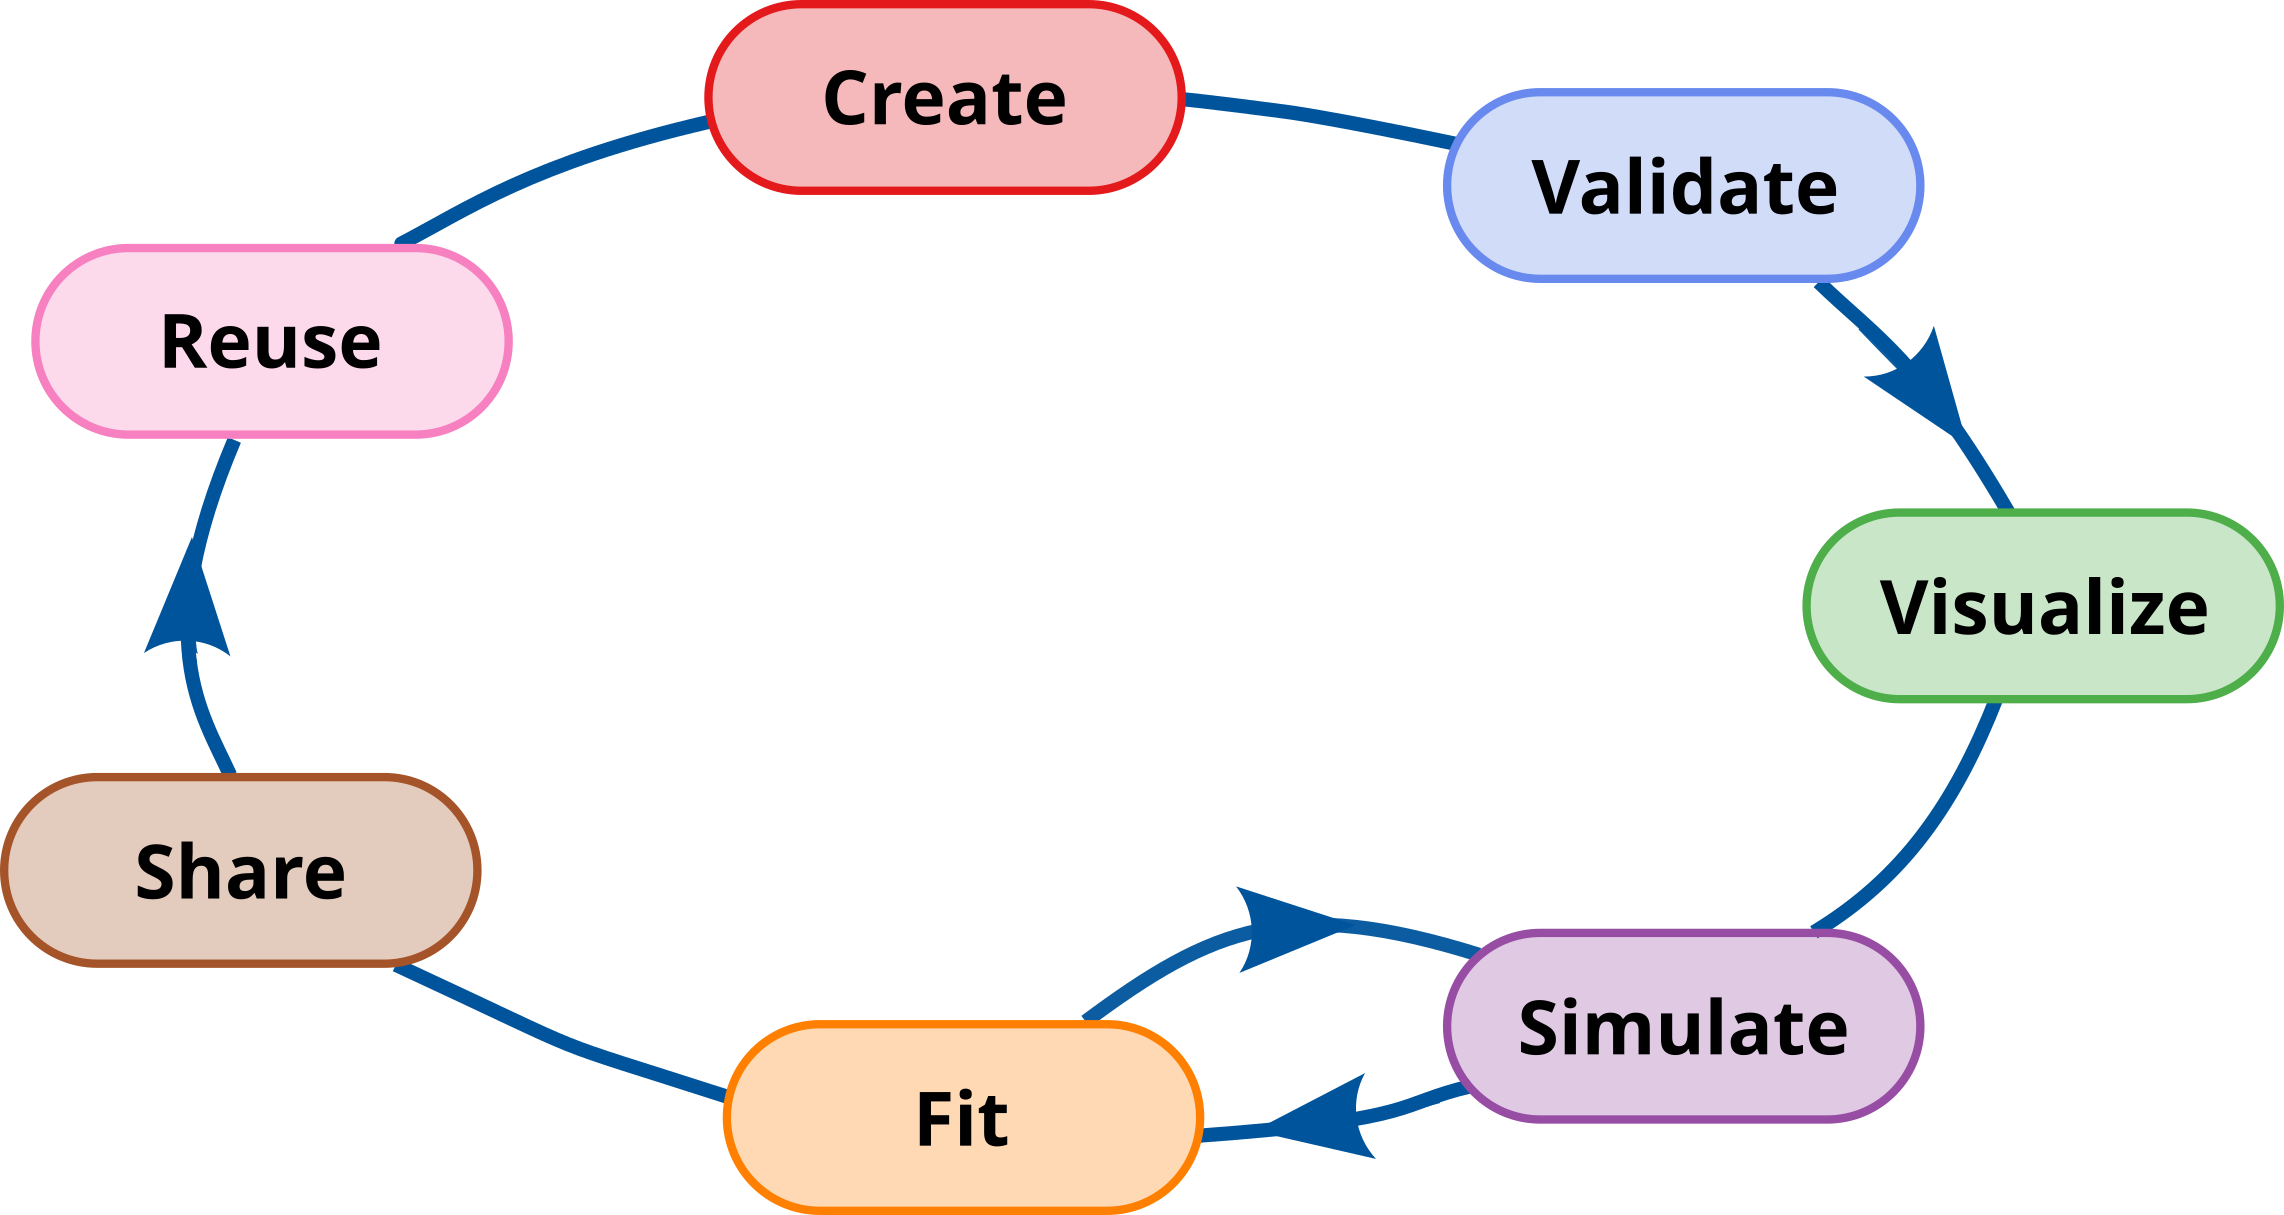
\includegraphics[width=\textwidth]{99_images/ecosystem-no-neuroml}
  \end{figure}
\note[item]{Ideally, what we want is for all the stages to be connected seamlessly, but this is not true in practice.}
\note[item]{We create our model, ideally re-using already published components.}
\note[item]{Then before we simulate our model, we want to validate it in some way.}
\note[item]{We also want to analyse and visualise our model description before.}
\note[item]{Then we iteratively simulate and fit our model to data, or to produce a certain behaviour.}
\note[item]{Finally, we want to publish and openly share the model so others can use it in the future.}
\end{frame}
\begin{frame}[c]
  \frametitle{Computational modelling software ecosystem is fragmented}
  \begin{itemize}
    \item many specialist tools:
      \begin{itemize}
        \item NEURON, NEST, Brian, GENESIS, MOOSE, STEPS, ANNarchy, TVB, LFPy, NeuroLib, EDEN, Arbor, NetPyNE\ldots{}
      \end{itemize}
    \item<2-> \alert{but:}
      \begin{itemize}
        \item<2-> different APIs, syntax:
          \begin{itemize}
            \item<2-> increased difficulty for users
          \end{itemize}
        \item<3-> not well defined model descriptions:
          \begin{itemize}
            \item<3-> models cannot be easily validated
          \end{itemize}
        \item<4-> custom machine readable internal representations:
          \begin{itemize}
            \item<4-> models cannot be easily inspected/analysed
          \end{itemize}
        \item<5-> ad-hoc utilities:
          \begin{itemize}
            \item<5->  cannot be used with all tools
          \end{itemize}
      \end{itemize}
  \end{itemize}
\note[item]{There are a lot of software tools out there for users to pick from, for different levels of modelling, optimisation, analysis.}
\note[item]{For each stage.}
\note[item]{But, they aren't designed to work together.}
\note[item]{They have their own designs, their own APIs, syntax, model representation, and usually their own suite of custom utilities to work with their model representation.}
\end{frame}
\begin{frame}[c]
  \frametitle{}
  \begin{center}
  \Large{Makes computational neuroscience models\\\emph{less}\\\alert{FAIR}\\\alert{(Findable, Accessible, Interoperable, Reusable)}}
  \end{center}
\note[item]{This means that for example, a model written in simulator A, say NEURON, cannot just be re-used in another simulator.}
\note[item]{In fact, because a majority of these tools do not have a well defined model description, even re-using models developed in the same simulator can be quite hard.}
\note[item]{It takes a lot of human resources to translate/convert models to be able to re-use them.}
\note[item]{It also makes it very hard to study or analyse these models.}
\end{frame}
\begin{frame}[c]
  \frametitle{Standards enable FAIR neuroscience}
  \begin{columns}
    \begin{column}{0.5\textwidth}
      \begin{figure}[h]
        \centering
        
\includegraphics[width=0.8\textwidth]{99_images/incf}\\\vspace{0.2cm}
        
\includegraphics[width=0.4\textwidth]{99_images/combine}\\
        \scriptsize{COMBINE}
      \end{figure}%
    \end{column}
    \uncover<2>{%
    \begin{column}{0.5\textwidth}
      \begin{figure}[h]
        \centering
        
\includegraphics[width=0.35\textwidth]{99_images/neuroml-logo}\\\vspace{0.5cm}
        
\includegraphics[width=0.35\textwidth]{99_images/NWB}\\\vspace{0.2cm}
        
\includegraphics[width=0.35\textwidth]{99_images/sbml}\\\vspace{0.2cm}
        
\includegraphics[width=0.35\textwidth]{99_images/sedml}
      \end{figure}%
    \end{column}}
  \end{columns}
  \footnotetext[1]{\fullcite{Abrams2022}: \url{https://incf.org}}
  \footnotetext[1]{COmputational Modeling in BIology NEtwork (COMBINE): \url{https://co.mbine.org/}}
\note[item]{Now, this isn't a problem unique to computational neuroscience, or even neuroscience.}
\note[item]{Multiple scientific fields have run into this issue, and the answer that they've all come up with is to standardise.}
\note[item]{Standards allow the representation of data and models in specific, agreed formats.}
\note[item]{Once a standard is agreed upon, everyone can target it---tools, representations, utilities.}
\note[item]{If one knows what the data is going to look like, one can then develop tools and APIs around it.}
\note[item]{And instead of everyone writing a tool for their own standard, every tool anyone writes for the one standard can be used with everyone's data.}
\end{frame}
%\section{NeuroML}
\begin{frame}[c]
  \frametitle{NeuroML ecosystem supports all stages of the model cycle}
  \begin{figure}[h]
    \centering
    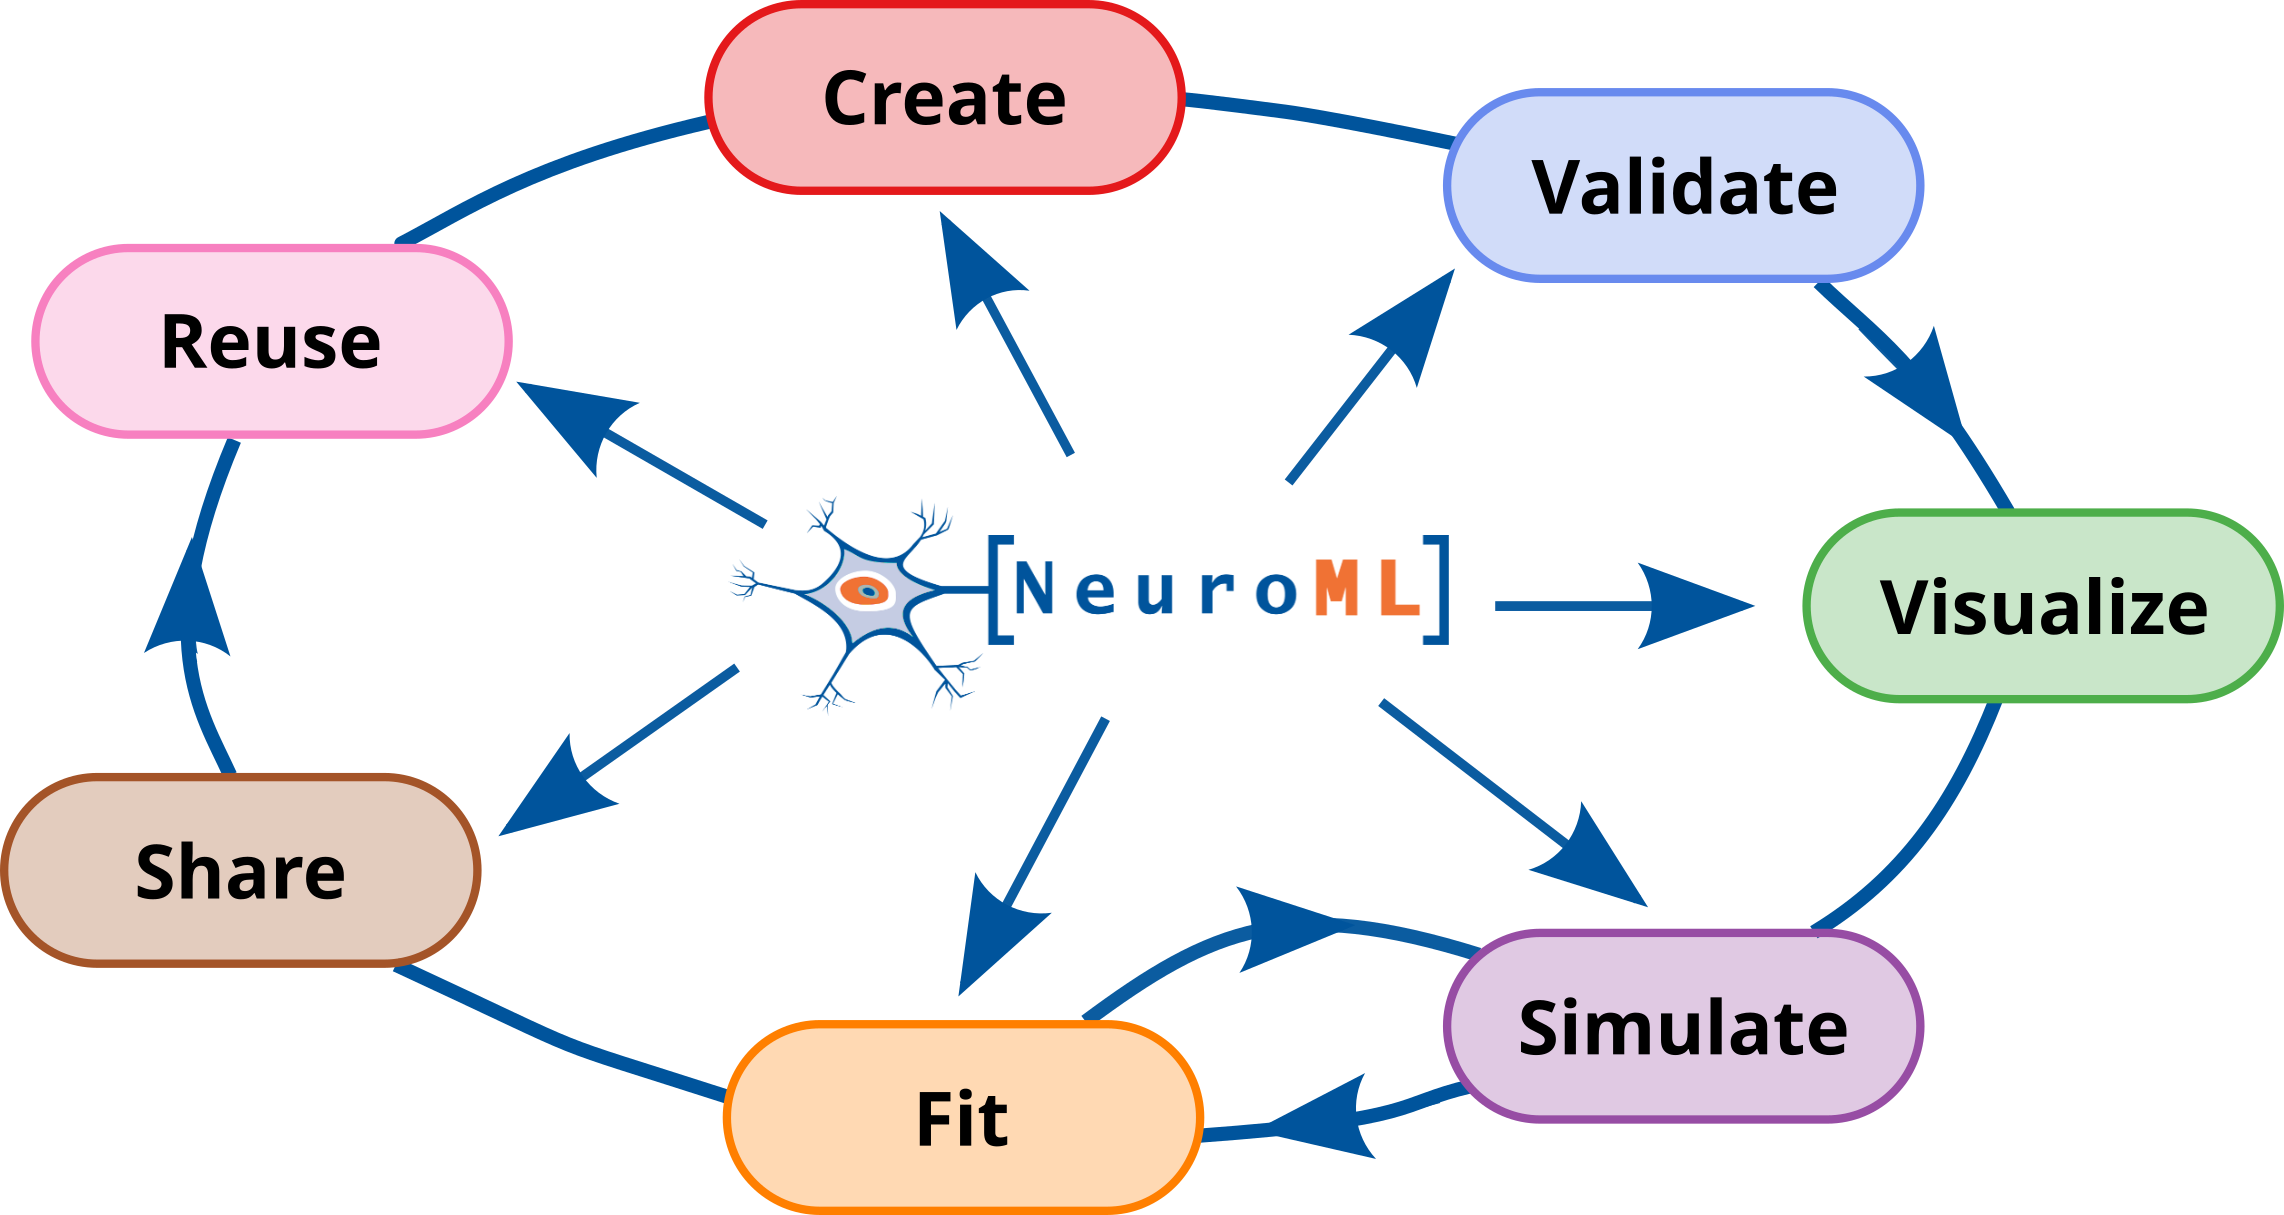
\includegraphics[width=\textwidth]{99_images/ecosystem}
  \end{figure}
\note[item]{The idea being that by being the standard, various tools that support various stages of the model life cycle can then work together.}
\end{frame}
\begin{frame}[c]
  \frametitle{NeuroML ecosystem}
  \begin{itemize}
    \item standard/specification
    \item software ecosystem
  \end{itemize}
\note[item]{It consists of two components. The specification or the standard, and the software that adhere to this specification.}
\end{frame}
\begin{frame}[t]
  \frametitle{NeuroML standard}
    Model specification (\alert{schema}: XSD)
    \begin{itemize}
      \item elements
      \item attributes
      \item hierarchical relationships
    \end{itemize}
  \uncover<2>{%
    Dynamics (\alert{LEMS component type definitions})
    \begin{itemize}
      \item dynamical behaviour
    \end{itemize}}
\note[item]{The standard itself has two different components.}
\note[item]{There's the schema, which formally specifies the model description---what elements, attributes are valid, and how they related to each other.}
\note[item]{The next is the LEMS description of the model---the dynamics. We call this the Component type declaration.}
\end{frame}
\begin{frame}[c]
  \frametitle{NeuroML standard: schema: XSD}
    Way of specifying the structure of an XML document.
    \begin{itemize}
      \item allows defining \alert{types} and \alert{extensions/restrictions} on types to create new types.
      \item allows generation of \alert{API}s
    \end{itemize}
    \pause{}
    \begin{center}
      \emph{A model description can be validated against the schema\\\alert{before simulation}}
    \end{center}
    \footnotetext[1]{\url{https://www.w3.org/TR/xmlschema-1/}}
\note[item]{That's it. We'll see an example now.}
\end{frame}
\begin{frame}[fragile,c]
  \frametitle{NeuroML standard: schema: XSD}
  \begin{center}
    \begin{minted}[breaklines=true,autogobble=True,fontsize=\Tiny,highlightlines={2,3}]{xml}
<xs:simpleType name="Nml2Quantity_voltage"> <!-- For params with dimension voltage -->
  <xs:restriction base="xs:string">
    <xs:pattern value="-?([0-9]*(\.[0-9]+)?)([eE]-?[0-9]+)?[\s]*(V|mV)"/>
  </xs:restriction>
</xs:simpleType>
    \end{minted}
    \pause{}
    \begin{minted}[breaklines=true,autogobble=True,fontsize=\Tiny,highlightlines={7,11}]{xml}
<xs:complexType name="Izhikevich2007Cell">
  <xs:annotation>
    <xs:documentation>Cell based on ...>
    </xs:documentation>
  </xs:annotation>
  <xs:complexContent>
    <xs:extension base="BaseCellMembPotCap">
      <xs:attribute name="v0" type="Nml2Quantity_voltage" use="required"/>
      <xs:attribute name="k" type="Nml2Quantity_conductancePerVoltage" use="required"/>
      <xs:attribute name="vr" type="Nml2Quantity_voltage" use="required"/>
      <xs:attribute name="vt" type="Nml2Quantity_voltage" use="required"/>
      <xs:attribute name="vpeak" type="Nml2Quantity_voltage" use="required"/>
      <xs:attribute name="a" type="Nml2Quantity_pertime" use="required"/>
      <xs:attribute name="b" type="Nml2Quantity_conductance" use="required"/>
      <xs:attribute name="c" type="Nml2Quantity_voltage" use="required"/>
      <xs:attribute name="d" type="Nml2Quantity_current" use="required"/>
    </xs:extension>
  </xs:complexContent>
</xs:complexType>
    \end{minted}
  \end{center}
  \footnotetext[1]{\fullcite{Izhikevich2007}}
\note[item]{The schema is defined as an XSD: XML schema document that formally defines what an XML file can look like.}
\note[item]{In this example, of a simple cell model, the Izhikevich model, this lists what its attributes are.}
\note[item]{In programming jargon, we're defining the structure of the class---what parameters/attributes can an instance/object of class contain.}
\end{frame}
\begin{frame}[t]
  \frametitle{NeuroML standard: LEMS component type definitions}
  \alert{L}ow \alert{E}ntropy \alert{M}odel \alert{S}pecification language
    \begin{itemize}
      \item domain independent
      \item allows creation of "Component Types" \alert{(classes)} from which "Components" \alert{(objects)} can be instantiated by providing the necessary parameters
      \item provides a \alert{reference implementation/simulator}
        \pause{}
      \item machine readable: \alert{translatable} into other formats
    \end{itemize}
    \footnotetext[1]{\fullcite{Cannon2014}}
\note[item]{The next is the LEMS description of the model---the dynamics. We call this the Component type declaration.}
\end{frame}
\begin{frame}[fragile,c]
  \frametitle{NeuroML standard: dynamics (LEMS)}
  \begin{center}
    \begin{minted}[breaklines=true,autogobble=True,fontsize=\Tiny,highlightlines={21,23,25}]{xml}
    <ComponentType name="izhikevich2007Cell" extends="baseCellMembPotCap"
        description="Cell based ...">

        <Parameter name="v0" dimension="voltage" description="Initial membrane potential"/>

        <!--
        Defined in baseCellMembPotCap:
        <Parameter name="C" dimension="capacitance"/>
        -->
        <Parameter name="k" dimension="conductance_per_voltage"/>

        <Parameter name="vr" dimension="voltage" description="Resting membrane potential"/>
        <Parameter name="vt" dimension="voltage" description="Spike threshold"/>
        <Parameter name="vpeak" dimension="voltage" description="Peak action potential value"/>

        <Parameter name="a" dimension="per_time" description="Time scale of recovery variable u"/>
        <Parameter name="b" dimension="conductance" description="Sensitivity of recovery variable u to subthreshold fluctuations of membrane potential v"/>
        <Parameter name="c" dimension="voltage" description="After-spike reset value of v"/>
        <Parameter name="d" dimension="current" description="After-spike increase to u"/>

        <Attachments name="synapses" type="basePointCurrent"/>

        <Exposure name="u" dimension="current" description="Membrane recovery variable"/>

        <Dynamics><!-- snipped --></Dynamics>

    </ComponentType>
    \end{minted}
  \end{center}
\note[item]{Here is the LEMS component type definition, without the dynamics for the moment.}
\note[item]{What you'll notice is that a lot of it is very similar to the XSD definition.}
\end{frame}
\begin{frame}[fragile,c]
  \frametitle{NeuroML standard: XSD and LEMS}
  XSD:
  \begin{center}
    \begin{minted}[breaklines=true,autogobble=True,fontsize=\Tiny,highlightlines={4,}]{xml}
      <xs:attribute name="v0" type="Nml2Quantity_voltage" use="required"/>
      <xs:attribute name="k" type="Nml2Quantity_conductancePerVoltage" use="required"/>
      <xs:attribute name="vr" type="Nml2Quantity_voltage" use="required"/>
      <xs:attribute name="vt" type="Nml2Quantity_voltage" use="required"/>
      <xs:attribute name="vpeak" type="Nml2Quantity_voltage" use="required"/>
      <xs:attribute name="a" type="Nml2Quantity_pertime" use="required"/>
      <xs:attribute name="b" type="Nml2Quantity_conductance" use="required"/>
      <xs:attribute name="c" type="Nml2Quantity_voltage" use="required"/>
      <xs:attribute name="d" type="Nml2Quantity_current" use="required"/>
    \end{minted}
  \end{center}
  LEMS:
  \begin{center}
    \begin{minted}[breaklines=true,autogobble=True,fontsize=\Tiny,highlightlines={4,}]{xml}
        <Parameter name="v0" dimension="voltage" description="Initial membrane potential"/>
        <Parameter name="k" dimension="conductance_per_voltage"/>
        <Parameter name="vr" dimension="voltage" description="Resting membrane potential"/>
        <Parameter name="vt" dimension="voltage" description="Spike threshold"/>
        <Parameter name="vpeak" dimension="voltage" description="Peak action potential value"/>
        <Parameter name="a" dimension="per_time" description="Time scale of recovery variable u"/>
        <Parameter name="b" dimension="conductance" description="Sensitivity of recovery variable u to subthreshold fluctuations of membrane potential v"/>
        <Parameter name="c" dimension="voltage" description="After-spike reset value of v"/>
        <Parameter name="d" dimension="current" description="After-spike increase to u"/>
    \end{minted}
  \end{center}
\note[item]{I've written the attributes/parameters together here so you can see that there's a one-to-one correspondence between the two model descriptions.}
\end{frame}
\begin{frame}[fragile,c]
  \frametitle{NeuroML standard: dynamics (LEMS)}
  \begin{center}
    \begin{minted}[breaklines=true,autogobble=True,fontsize=\Tiny]{xml}
    <ComponentType name="izhikevich2007Cell" extends="baseCellMembPotCap"
        description="Cell based ...">
        <!-- snipped -->
        <Attachments name="synapses" type="basePointCurrent"/>

        <Exposure name="u" dimension="current" description="Membrane recovery variable"/>

        <Dynamics>
            <StateVariable name="v" dimension="voltage" exposure="v"/>
            <StateVariable name="u" dimension="current" exposure="u"/>

            <DerivedVariable name="iSyn"  dimension="current" exposure="iSyn" select="synapses[*]/i" reduce="add" />

            <DerivedVariable name="iMemb" dimension="current" exposure="iMemb" value="k * (v-vr) * (v-vt) + iSyn - u"/>

            <TimeDerivative variable="v" value="iMemb / C"/>
            <TimeDerivative variable="u" value="a * (b * (v-vr) - u)"/>

            <OnStart>
                <StateAssignment variable="v" value="v0"/>
                <StateAssignment variable="u" value="0"/>
            </OnStart>

            <OnCondition test="v .gt. vpeak">
                <StateAssignment variable="v" value="c"/>
                <StateAssignment variable="u" value="u + d"/>
                <EventOut port="spike"/>
            </OnCondition>

        </Dynamics>
    </ComponentType>
    \end{minted}
  \end{center}
\note[item]{This now shows the dynamics of the component type.}
\note[item]{It include information on how the states and time derivatives change, how the various variables interact.}
\note[item]{This information is sufficient to then be able to create an object of this type and to simulate it.}
\end{frame}
\begin{frame}[c]
  \frametitle{NeuroML is declarative, modular, structured, hierarchical}
  \begin{columns}
    \begin{column}{0.3\textwidth}
      \begin{figure}[h]
        \centering
        Conductances\\
        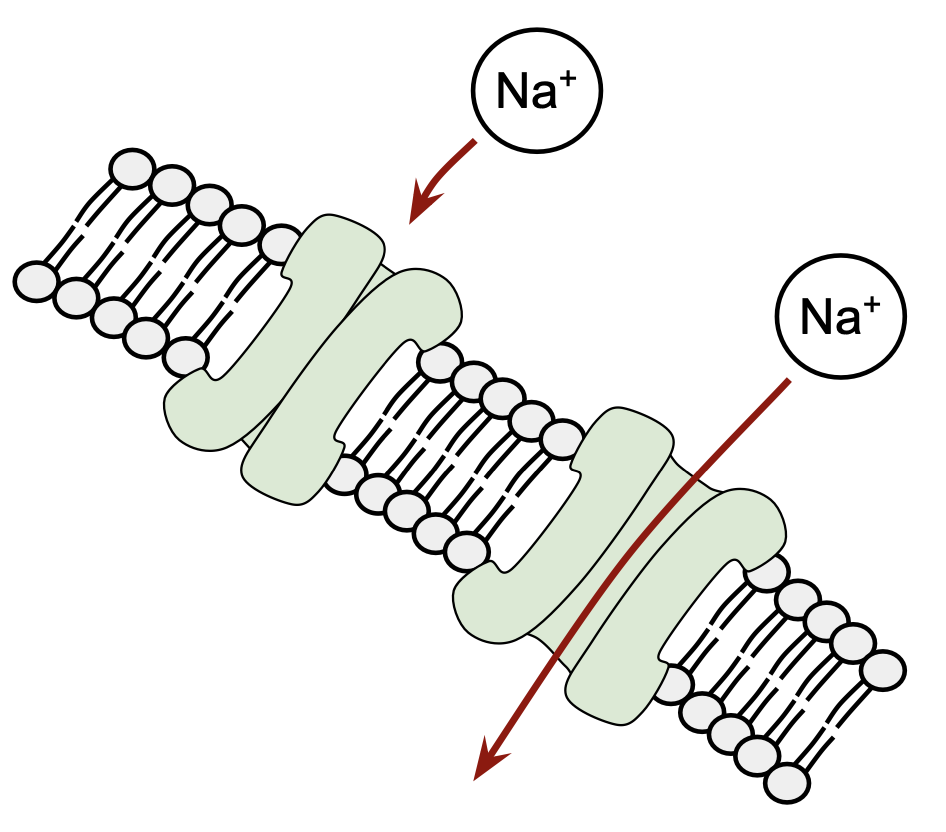
\includegraphics[width=0.7\textwidth]{99_images/membrane2}\\\vspace{0.2cm}
      \end{figure}%
    \end{column}
    \begin{column}{0.3\textwidth}
      \begin{figure}[h]
        \centering
        Cells\\\vspace{-0.5cm}
        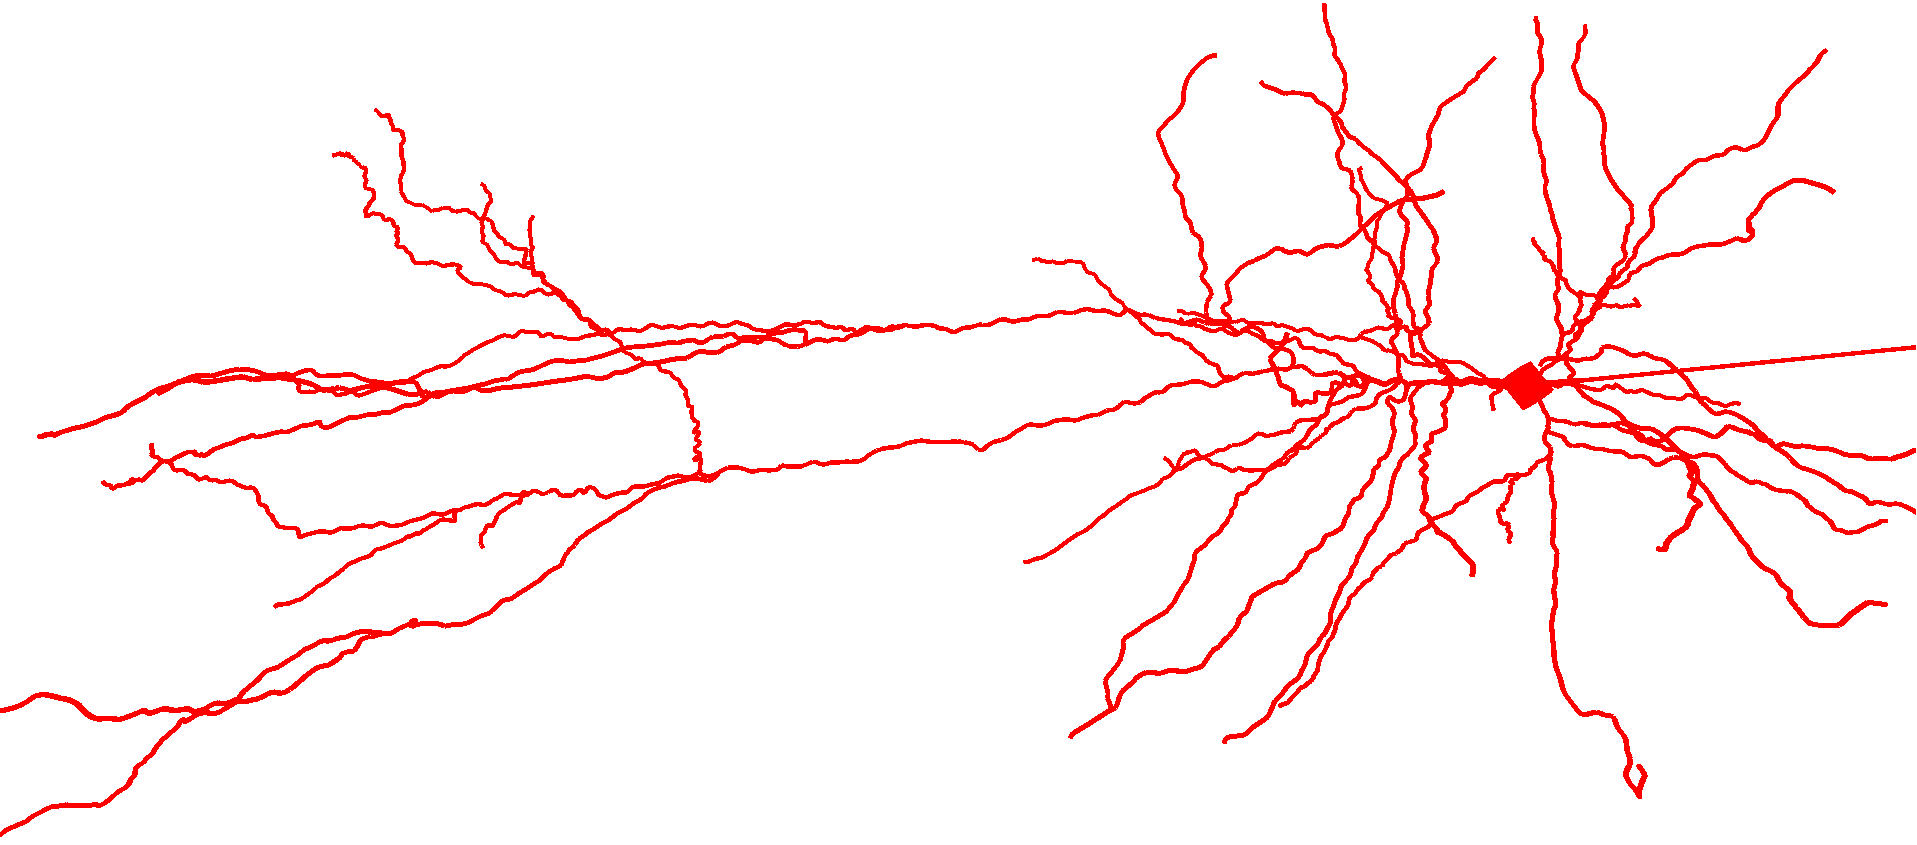
\includegraphics[width=0.7\textwidth,angle=-90]{99_images/HL23PYR-red}
        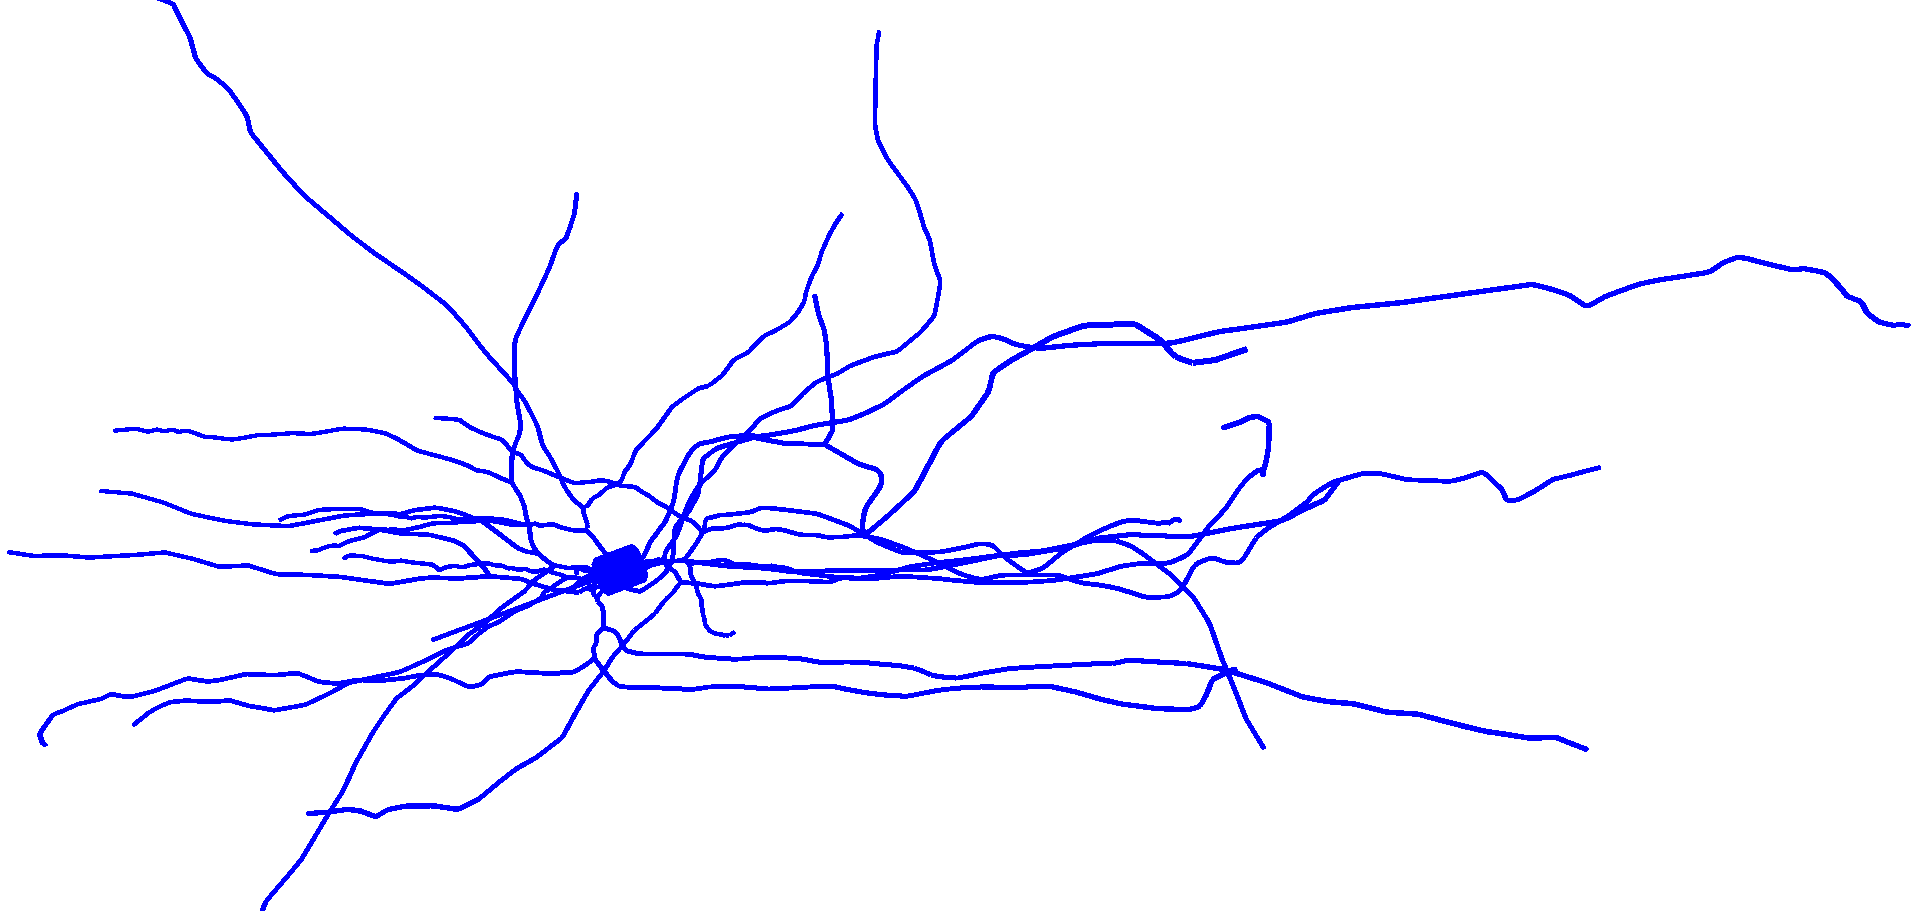
\includegraphics[width=0.7\textwidth,angle=-90]{99_images/HL23PV}
      \end{figure}%
    \end{column}
    \begin{column}{0.3\textwidth}
      \begin{figure}[h]
        \centering
        Networks\\
        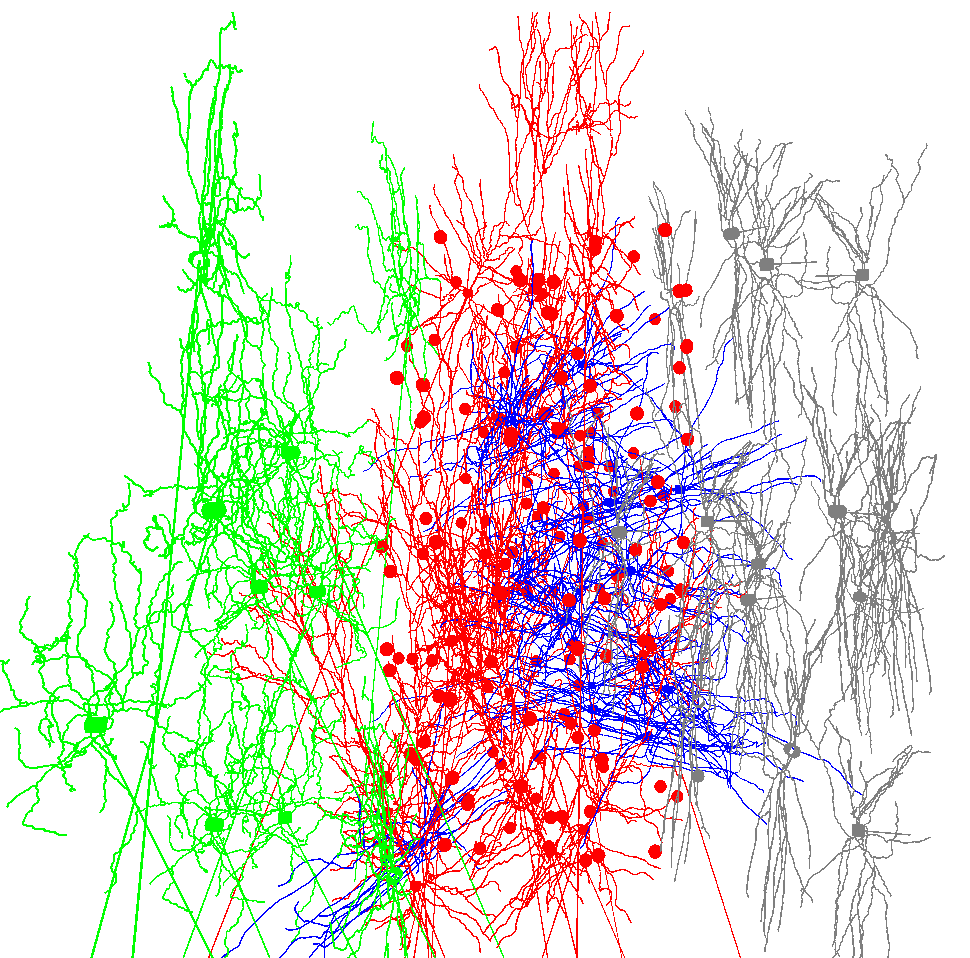
\includegraphics[width=0.7\textwidth]{99_images/20231004-HL23Net}\\\vspace{0.2cm}
      \end{figure}%
    \end{column}
  \end{columns}
  \begin{figure}[h]
    \centering
    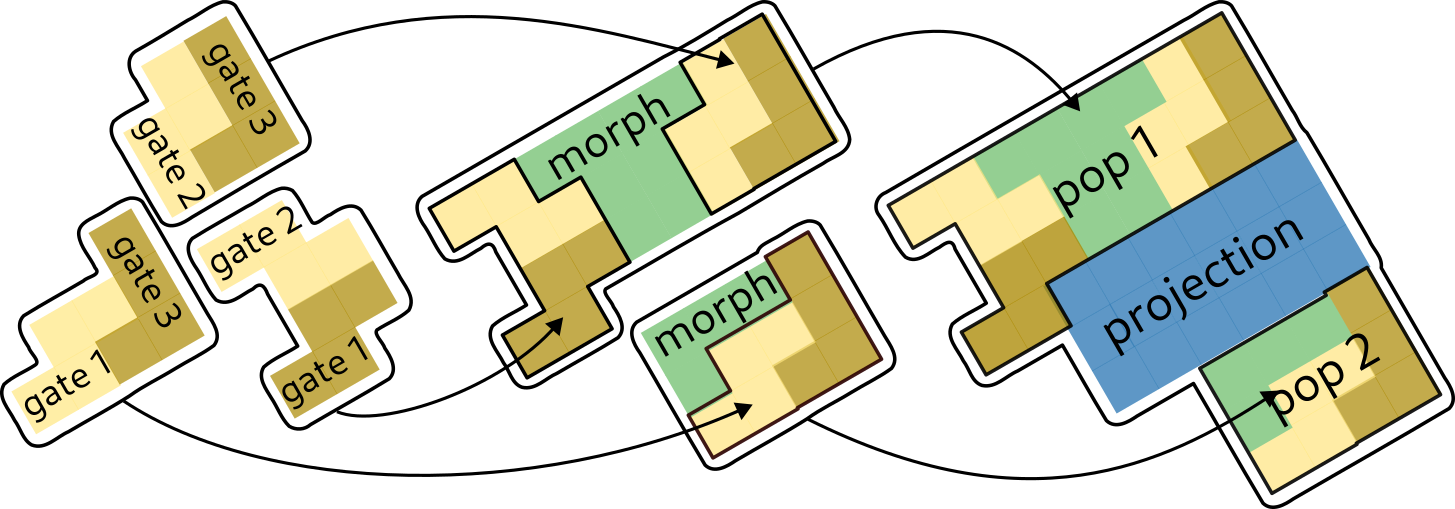
\includegraphics[width=0.9\textwidth]{99_images/lego}
  \end{figure}%
\note[item]{Hopefully this gives you an idea of how NeuroML is modular, structured, and hierarchical by design.}
\note[item]{So, we like to think of it building blocks, and since the relationships between blocks is well defined, the blocks can be easily re-used and combined to create new ones.}
\note[item]{So, there are three conductances here, for example---using the same three HH type gates.}
\note[item]{These conductances can be used in different cells---here two cells with different morphologies.}
\note[item]{The cells can then be used in populations to create a network, and so on.}
\end{frame}
\begin{frame}[c]
  \frametitle{NeuroML provides users with a set of curated model elements}
  \begin{figure}[h]
    \centering
    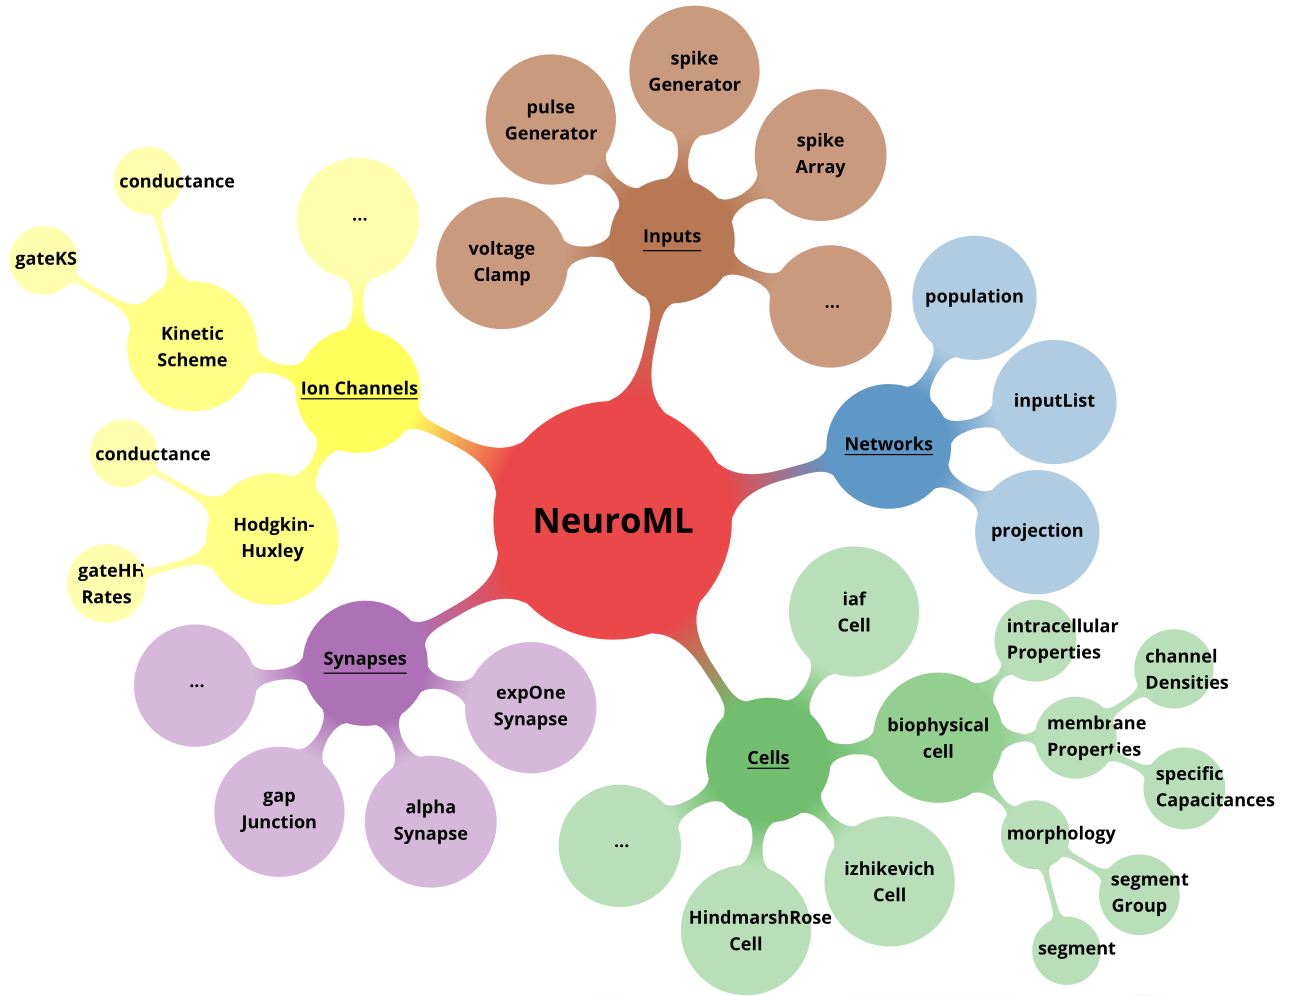
\includegraphics[width=0.9\textwidth]{99_images/neuroml-mindmap}
  \end{figure}%
  \footnotetext[1]{Full standard is at:~\url{https://docs.neuroml.org/Userdocs/Specification.html}}
\note[item]{An important aspect of the standard is that it includes lots of commonly used model elements already.}
\note[item]{So that users don't have to write these themselves, they can use the ones already provided.}
\note[item]{The mind map shows you a sub-set of model elements included in the NeuroML standard.}
\end{frame}
\begin{frame}[c]
  \frametitle{NeuroML software ecosystem}
  \begin{figure}[t]
    \begin{figure}[h]
      \centering
      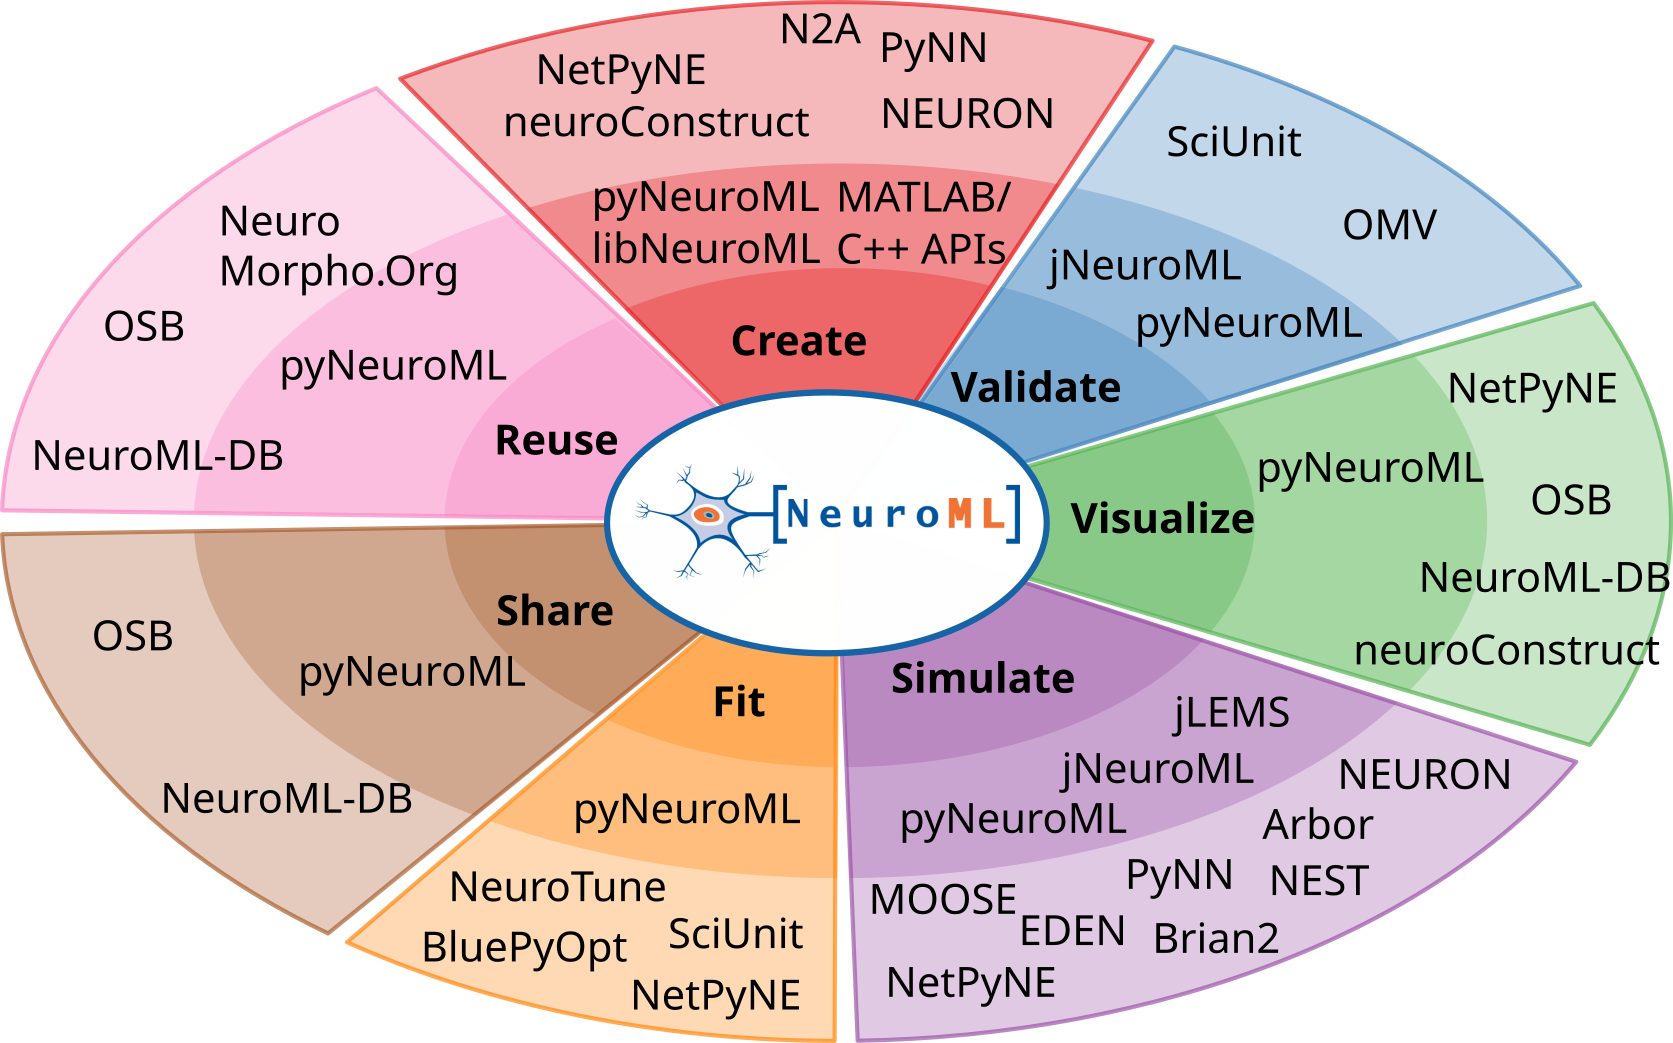
\includegraphics[width=0.9\textwidth]{99_images/ecosystem-onion}
    \end{figure}%
  \end{figure}
\note[item]{An important aspect of the standard is that it includes lots of commonly used model elements already.}
\note[item]{So that users don't have to write these themselves, they can use the ones already provided.}
\note[item]{The mind map shows you a sub-set of model elements included in the NeuroML standard.}
\end{frame}
\begin{frame}[c]
  \frametitle{NeuroML software ecosystem: core tools}
  \begin{figure}[h]
    \centering
    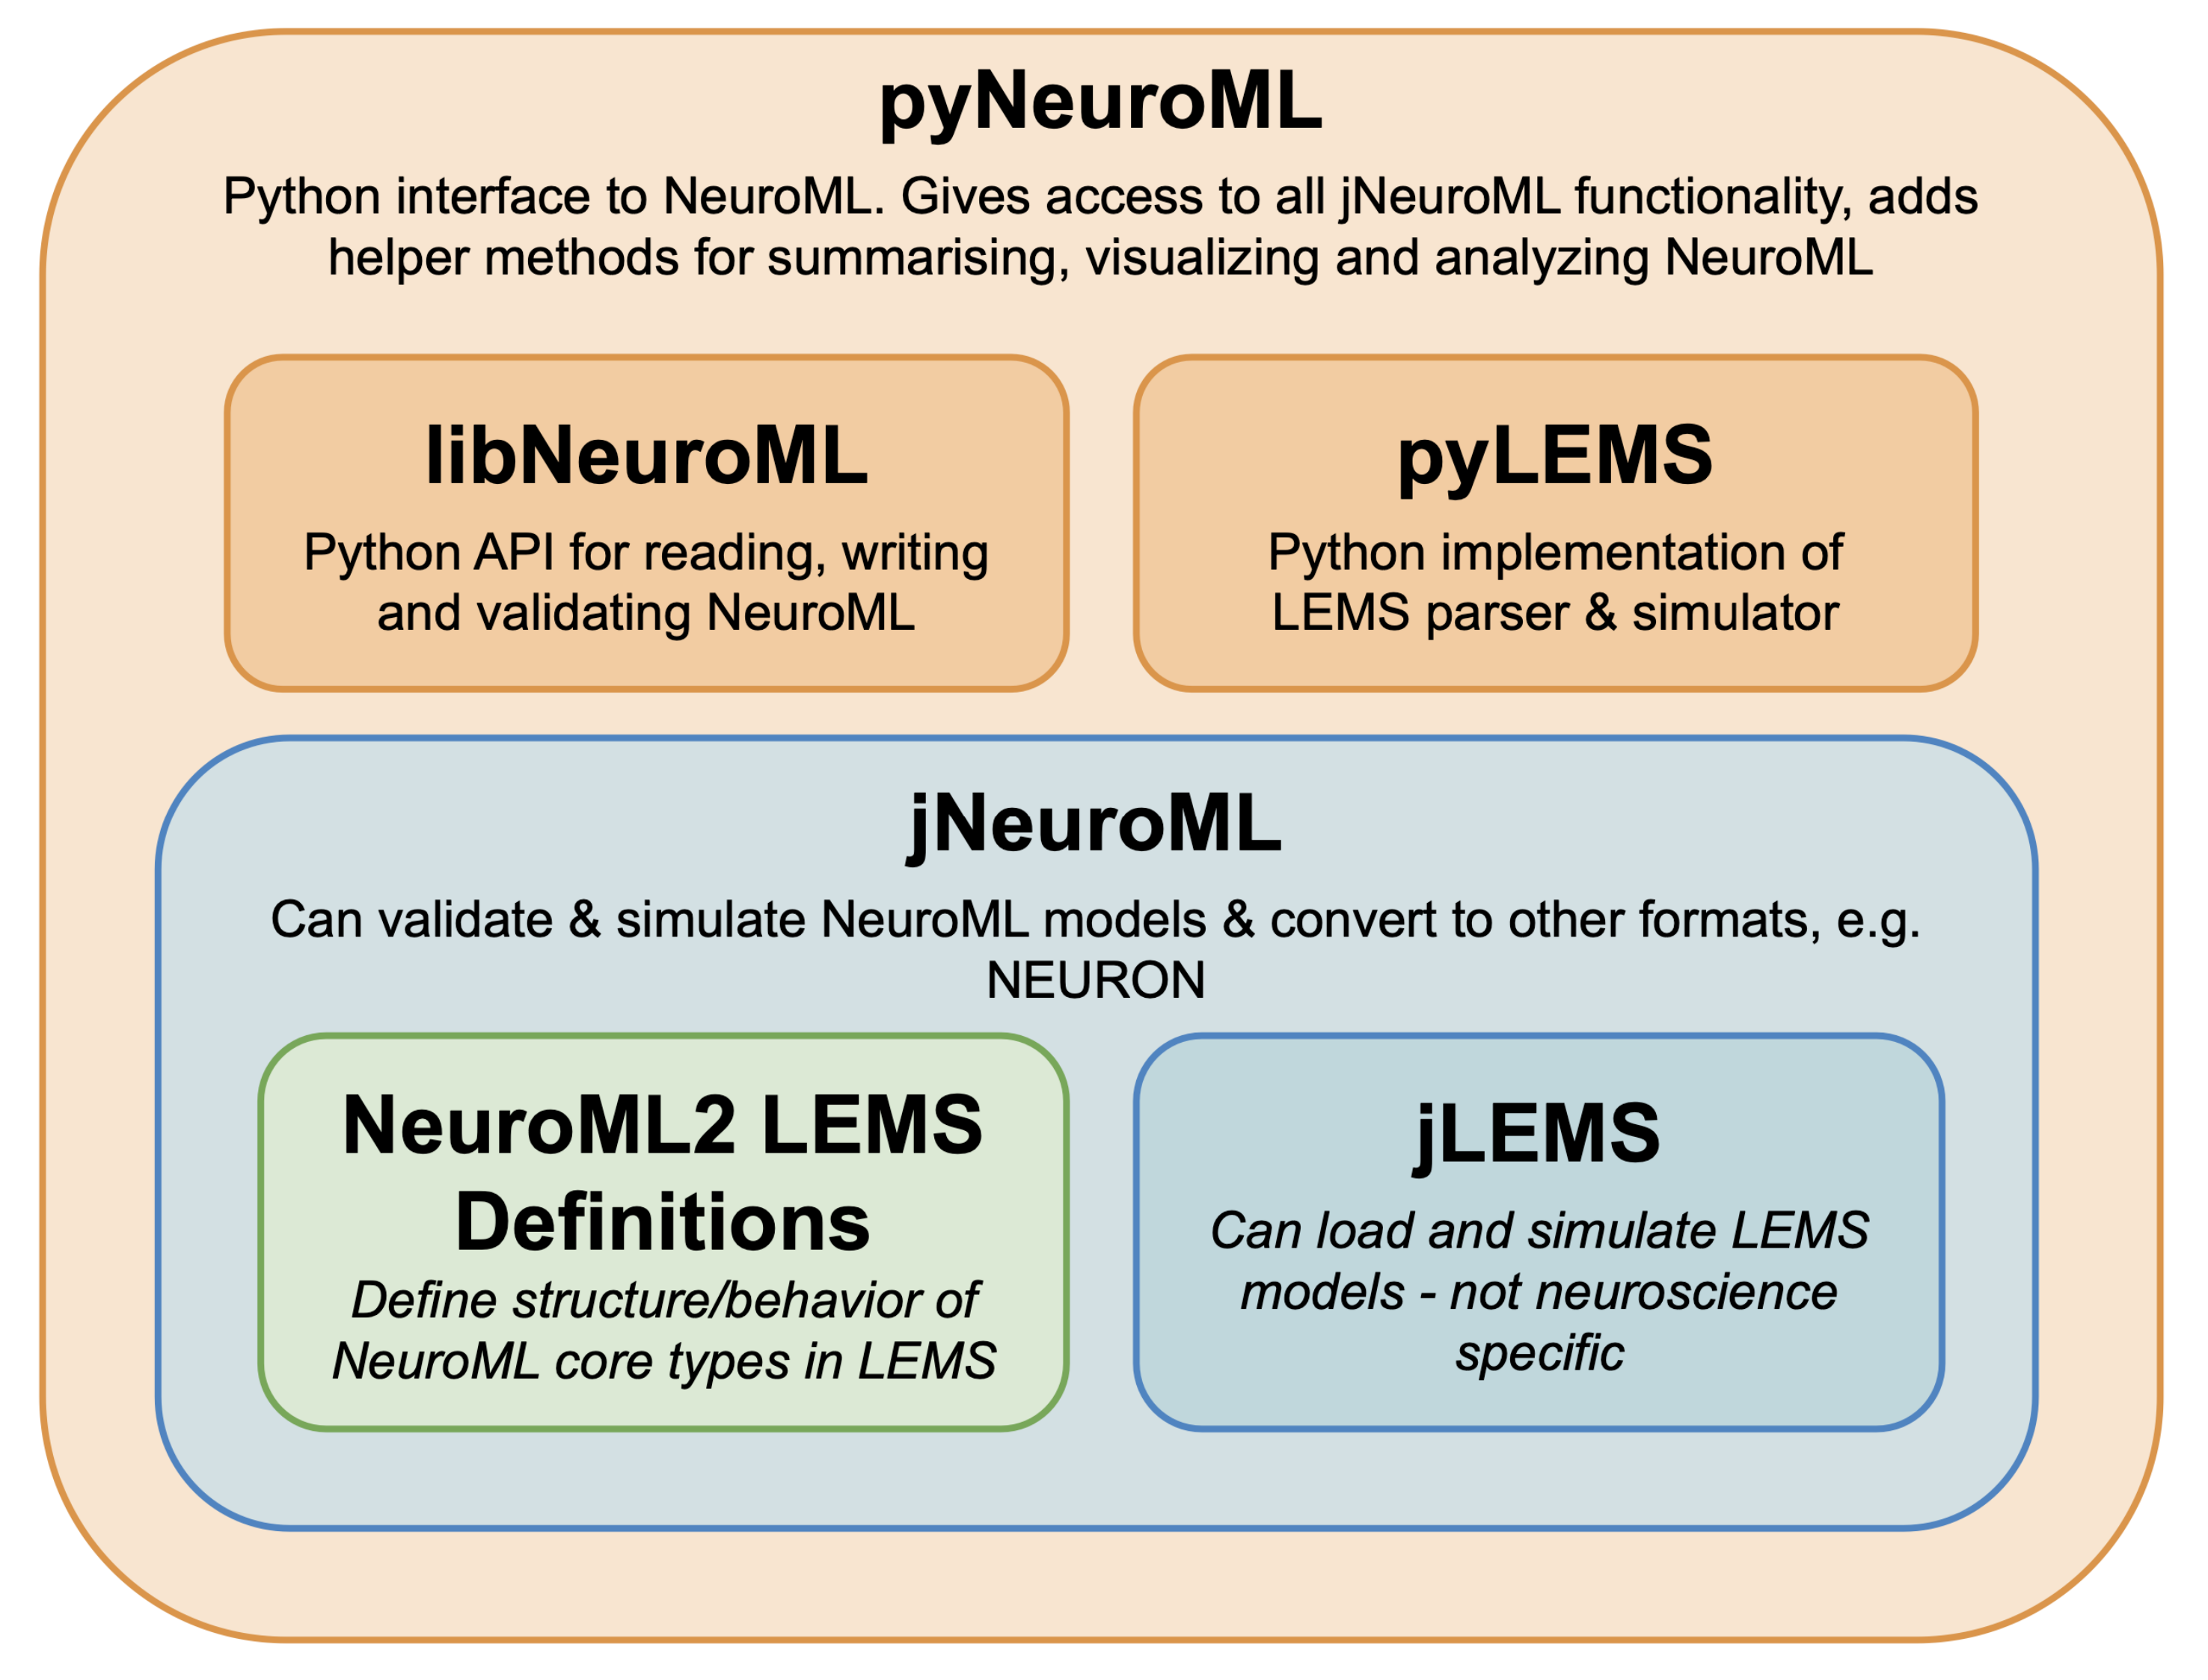
\includegraphics[width=0.8\textwidth]{99_images/software.png}
  \end{figure}
  \begin{center}
    \texttt{pip install pyneuroml}
  \end{center}
  \note[item]{These tools form the core NeuroML tools---ones that the NeuroML Editors, we develop and maintain}
  \note[item]{These provide the basic APIs required to work with NeuroML models---to create them, to read, write, and modify them}
  \note[item]{PyNeuroML is the suggested tool for use---we don't want people writing XML.}
\end{frame}
\begin{frame}[fragile,t]
  \frametitle{NeuroML software ecosystem: pyNeuroML}
  \begin{columns}
    \begin{column}{0.5\textwidth}
      \begin{minted}[breaklines=true,fontsize=\Tiny,breaksymbolleft={},breakindentnchars=4,autogobble]{python}
    # validation
    validate_neuroml2("file.nml")
    doc.validate(recursive=True)

    # inspection
    element.info()
    summary(doc)
    nml2_to_png(doc)
    nml2_to_svg(doc)
    generate_nmlgraph(doc)

    # visualisation/analysis
    plot_2D(cell)
    plot_interactive_3d(cell)
    plot_interactive_3d(network)

    plot_channel_densities(cell)
    plot_time_series(file)


    # simulation
    run_lems_with_jneuroml("sim.xml")
    run_lems_with_jneuroml_neuron("sim.xml")
    run_on_nsg("jneuroml_neuron", "sim.xml")

    # sharing
    create_combine_archive("sim.xml")
      \end{minted}
    \end{column}
    \begin{column}{0.5\textwidth}
      \begin{minted}[breaklines=true,fontsize=\Tiny,breaksymbolleft={},breakindentnchars=4,autogobble]{console}
    $ pynml "file.nml" -validate



    $ pynml-summary "file.nml"
    $ pynml -png "file.nml"
    $ pynml -svg "file.nml"
    $ pynml "file.nml" -graph
    $ pynml "file.nml" -matrix 1
    $ pynml-plotmorph "cell.nml"
    $ pynml-plotmorph -i "cell.nml"
    $ pynml-plotmorph -i "network.nml"
    $ pynml-channelanalysis "channel.nml"
    $ pynml-plotchan "channel.nml"
    $ pynml-plotspikes "sim.xml"
    $ pynml-plottimeseries "sim.xml"
    $ pynml-plottimeseries "*.dat"



    $ pynml "siml.xml"
    $ pynml "siml.xml" -neuron -run



    $ pynml-archive "file.xml"
      \end{minted}
    \end{column}
  \end{columns}
  \note[item]{PyNeuroML is the suggested tool for use---we don't want people writing XML.}
  \note[item]{PyNeuroML includes functions to support the model life cycle}
  \note[item]{These can be accessed programmatically, but we also provide CLIs to make it easier for users.}
\end{frame}
\begin{frame}[fragile,c]
  \frametitle{NeuroML: creating/simulating models}
  Python script to create a new network, and validate it:
    \begin{minted}[breaklines=true,fontsize=\Tiny,breaksymbolleft={},breakindentnchars=4,autogobble]{python}
    from neuroml import * # NeuroML API libNeuroML

    newdoc = NeuroMLDocument(id="new_doc")
    newcell = IafTauCell(id="cell_0", leak_reversal="-60mV", thresh="0mV", tau="5ms", reset="-70mV")
    newdoc.add(newcell)

    network = newdoc.add(Network, id="new_net", validate=False)
    population = network.add(Population, id="new_pop", size=10, component=newcell.id)

    # Helper method to ensure all parameters
    # present and appropriate
    newdoc.validate(recursive=True)
    \end{minted}
    Resultant NeuroML XML serialization:
    \begin{minted}[breaklines=true,fontsize=\Tiny,breaksymbolleft={},breakindentnchars=4,autogobble]{xml}
<neuroml id="new_doc">
  <iafTauCell id="cell_0" leakReversal="-60mV" thresh="0mV" reset="-70mV" tau="5ms"/>
  <network id="new_net">
      <population id="new_pop" component="cell_0" size="10"/>
  </network>
</neuroml>
    \end{minted}
    \note[item]{Now, we do not want users to write XML at all}
    \note[item]{The Python API is generated from the schema, and one can use this to write models.}
\end{frame}
\begin{frame}[c]
  \frametitle{NeuroML: creating/simulating models}
  \begin{figure}[h]
    \centering
    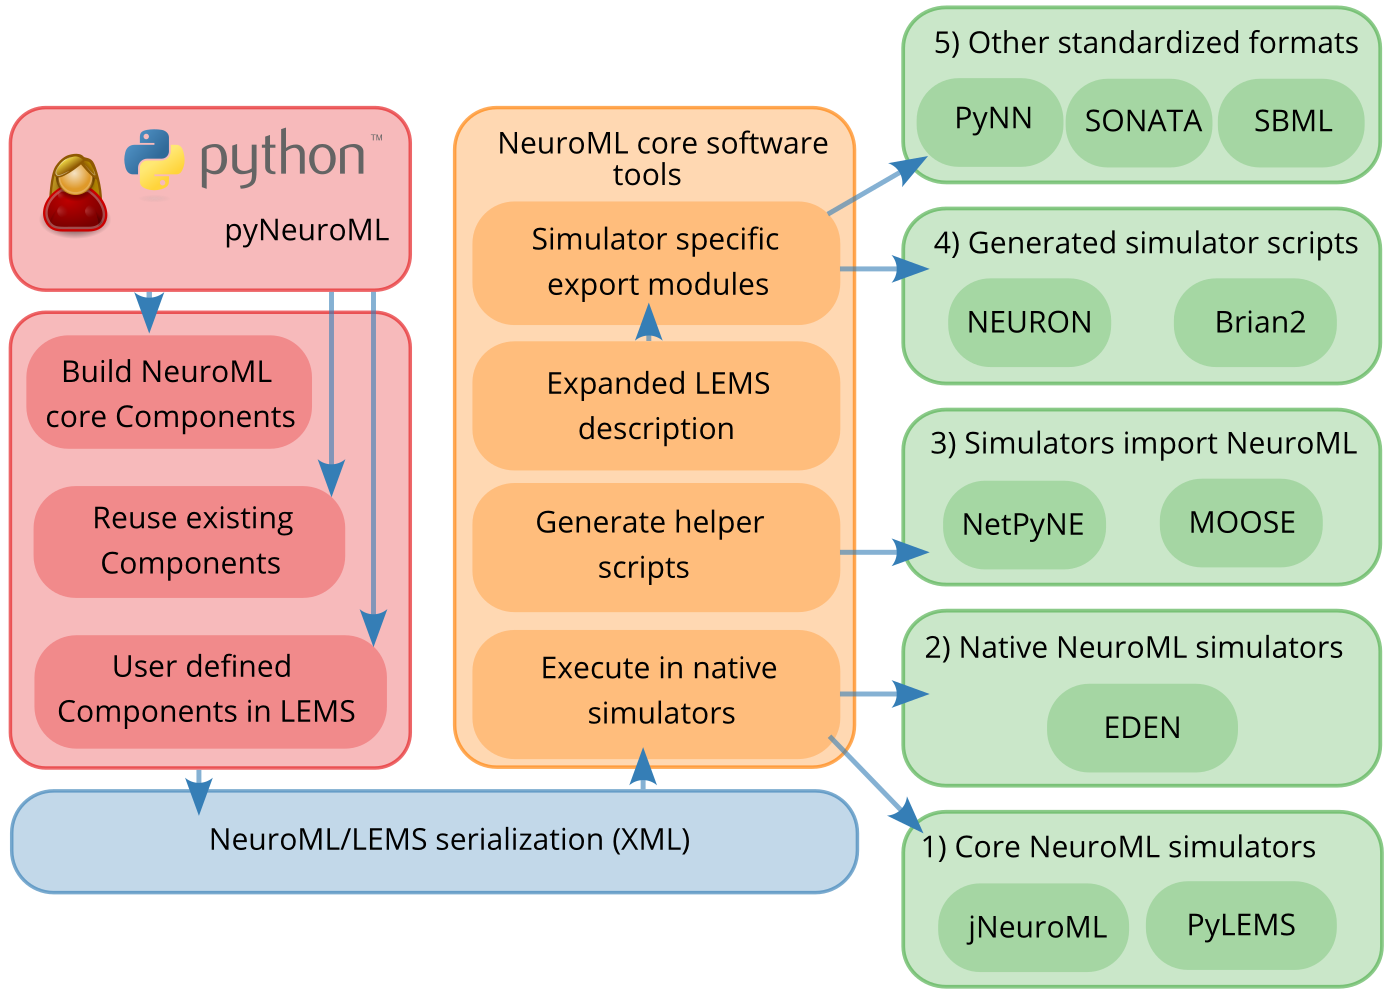
\includegraphics[width=0.9\textwidth]{99_images/create-translate-schematic}
  \end{figure}
  \note[item]{Once a model has been created, it is stored in its NeuroML/LEMS XML form}
  \note[item]{Because LEMS is formally defined and machine readable, this can now be easily converted into any other require format}
  \note[item]{The different simulators support NeuroML in different ways}
  \note[item]{For example, for NEURON, we generate NEURON scripts}
  \note[item]{But NetPyNE imports NeuroML to convert it into its own internal format}
  \note[item]{The advantage here is that simulator developers are free to choose how they want to support NeuroML}
\end{frame}
\begin{frame}[t]
  \frametitle{NeuroML: validating models}
  \begin{figure}[h]
    \only<1>{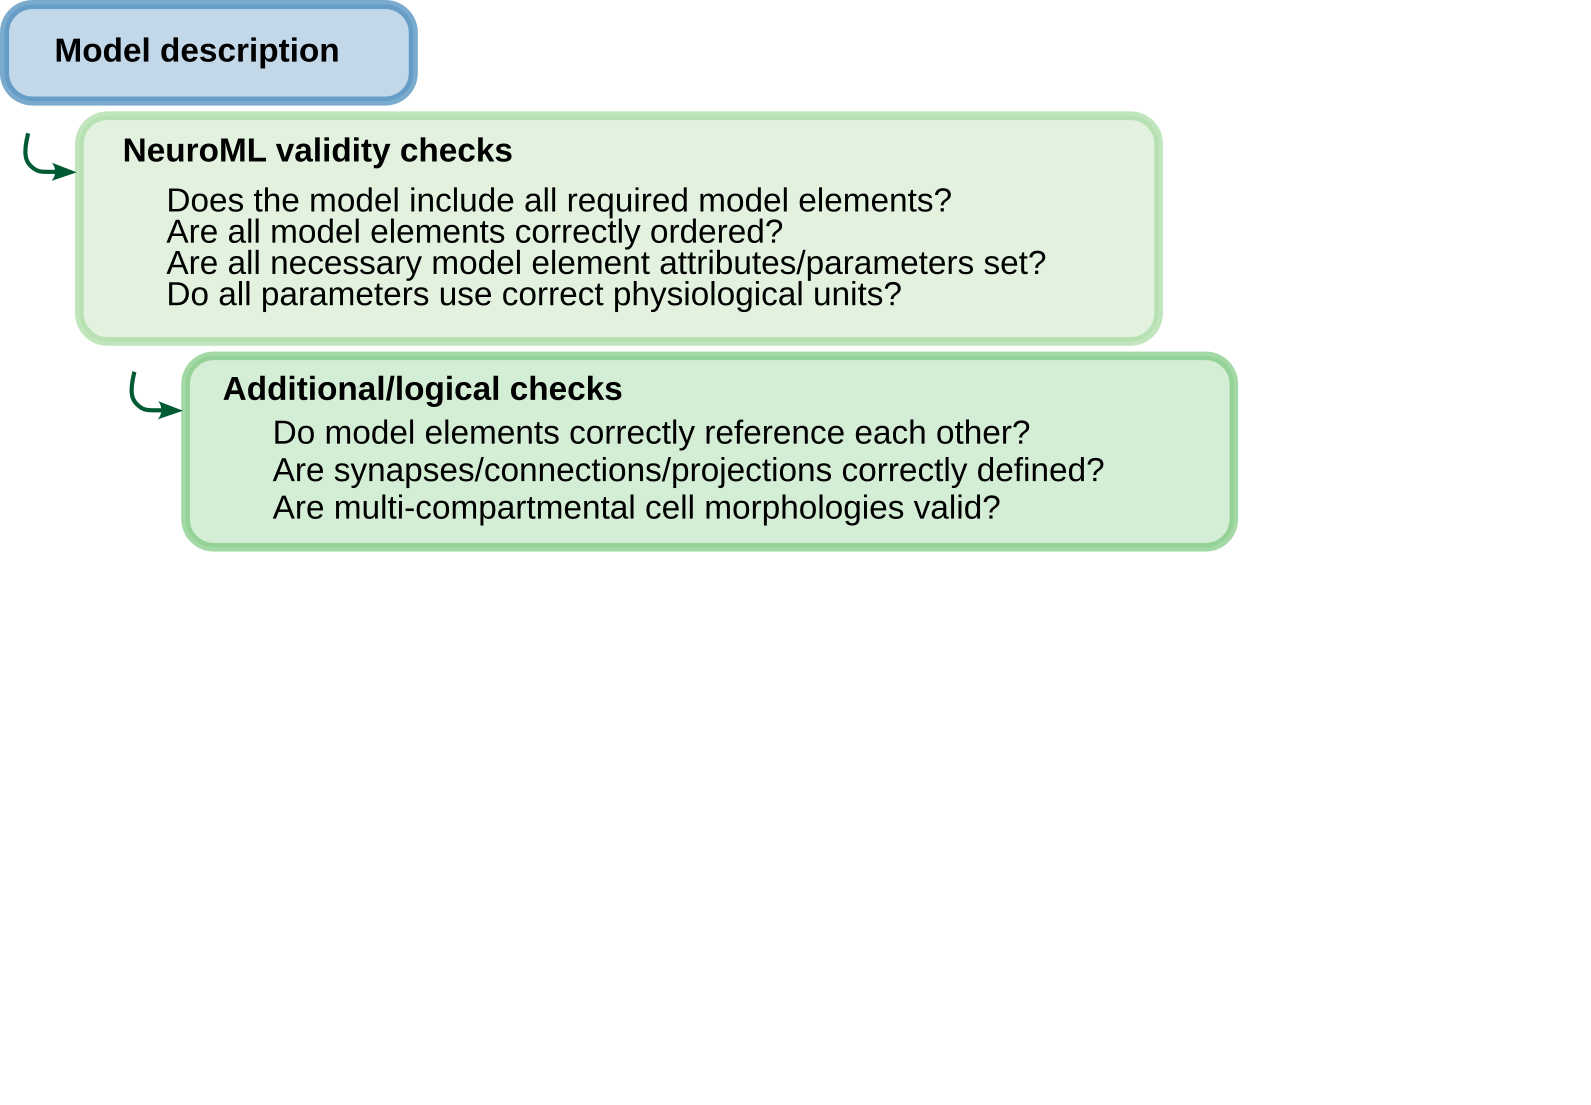
\includegraphics[width=0.8\textwidth]{99_images/validation-schematic-1}}%
    \only<2>{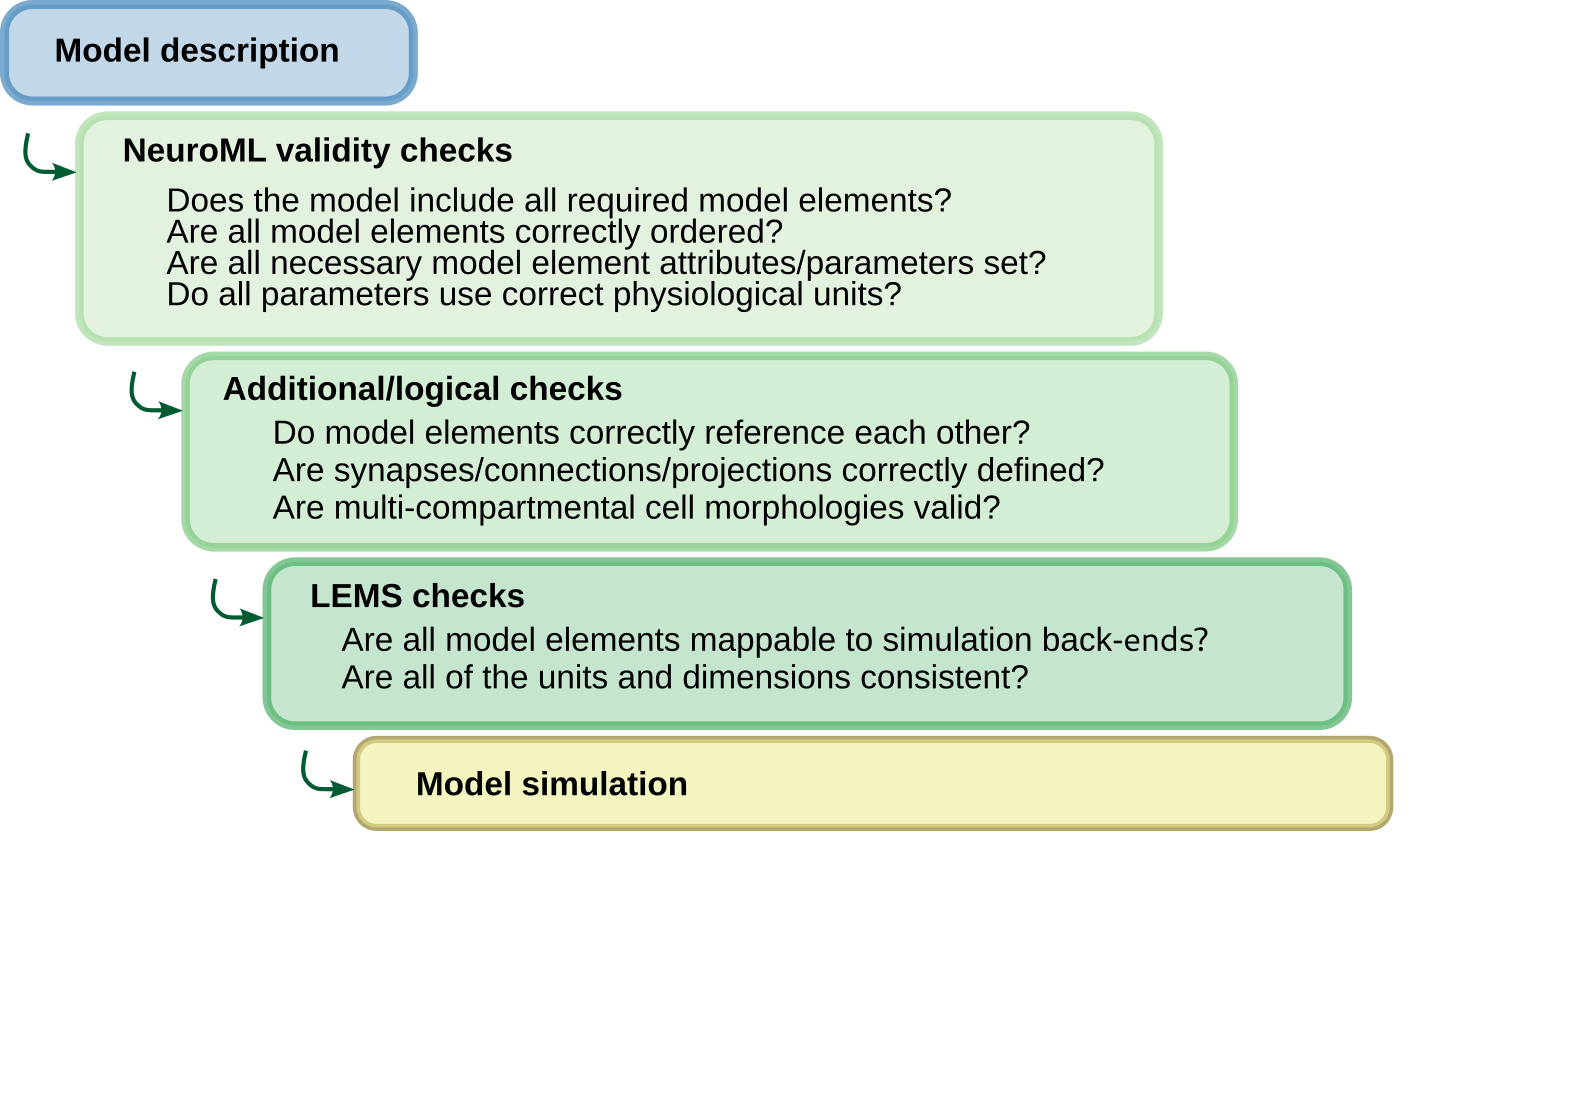
\includegraphics[width=0.8\textwidth]{99_images/validation-schematic-2}}%
    \only<3>{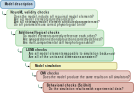
\includegraphics[width=0.8\textwidth]{99_images/validation-schematic}}%
  \end{figure}
  \only<3>{\footnotetext[1]{\url{https://github.com/OpenSourceBrain/osb-model-validation}}}
  \only<3>{\footnotetext[1]{\url{https://sciunit.io}}}
  \note[item]{We've already touched on validation a little, but let's look at it in more detail}
  \note[item]{The first level of validation is against the schema---is the model valid, does it have the right structure}
  \note[item]{Since we have access to the complete model description, we can also run additional global checks---are connections correctly defined, for example?}
  \note[item]{Once the model has been converted to its expanded LEMS form, we run more checks}
  \note[item]{Does the model support the requested simulator?}
  \note[item]{LEMS is dimension aware---so it checks to see if units and dimensions are consistent}
  \note[item]{We can now simulate the model being fairly confident that it has been defined correctly}
  \note[item]{We can then run more tests---do we get the same results everywhere? Does it produce the right behaviour?}
\end{frame}
\begin{frame}[c]
  \frametitle{NeuroML: visualising/analysing models}
  \begin{figure}[h]
    \only<1>{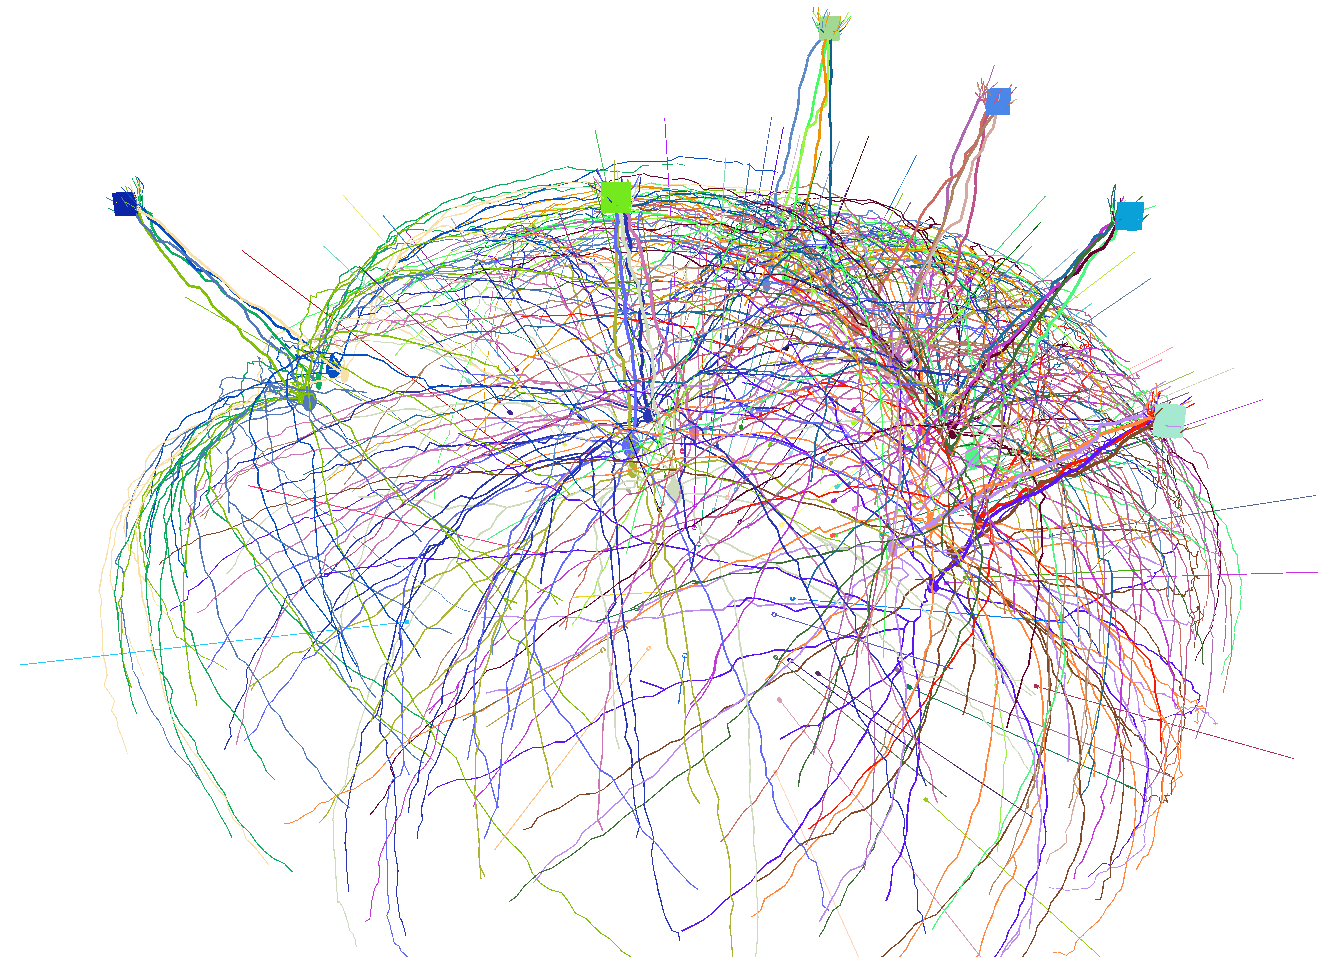
\includegraphics[width=0.9\textwidth]{99_images/20231004-migliore}}%
    \only<2>{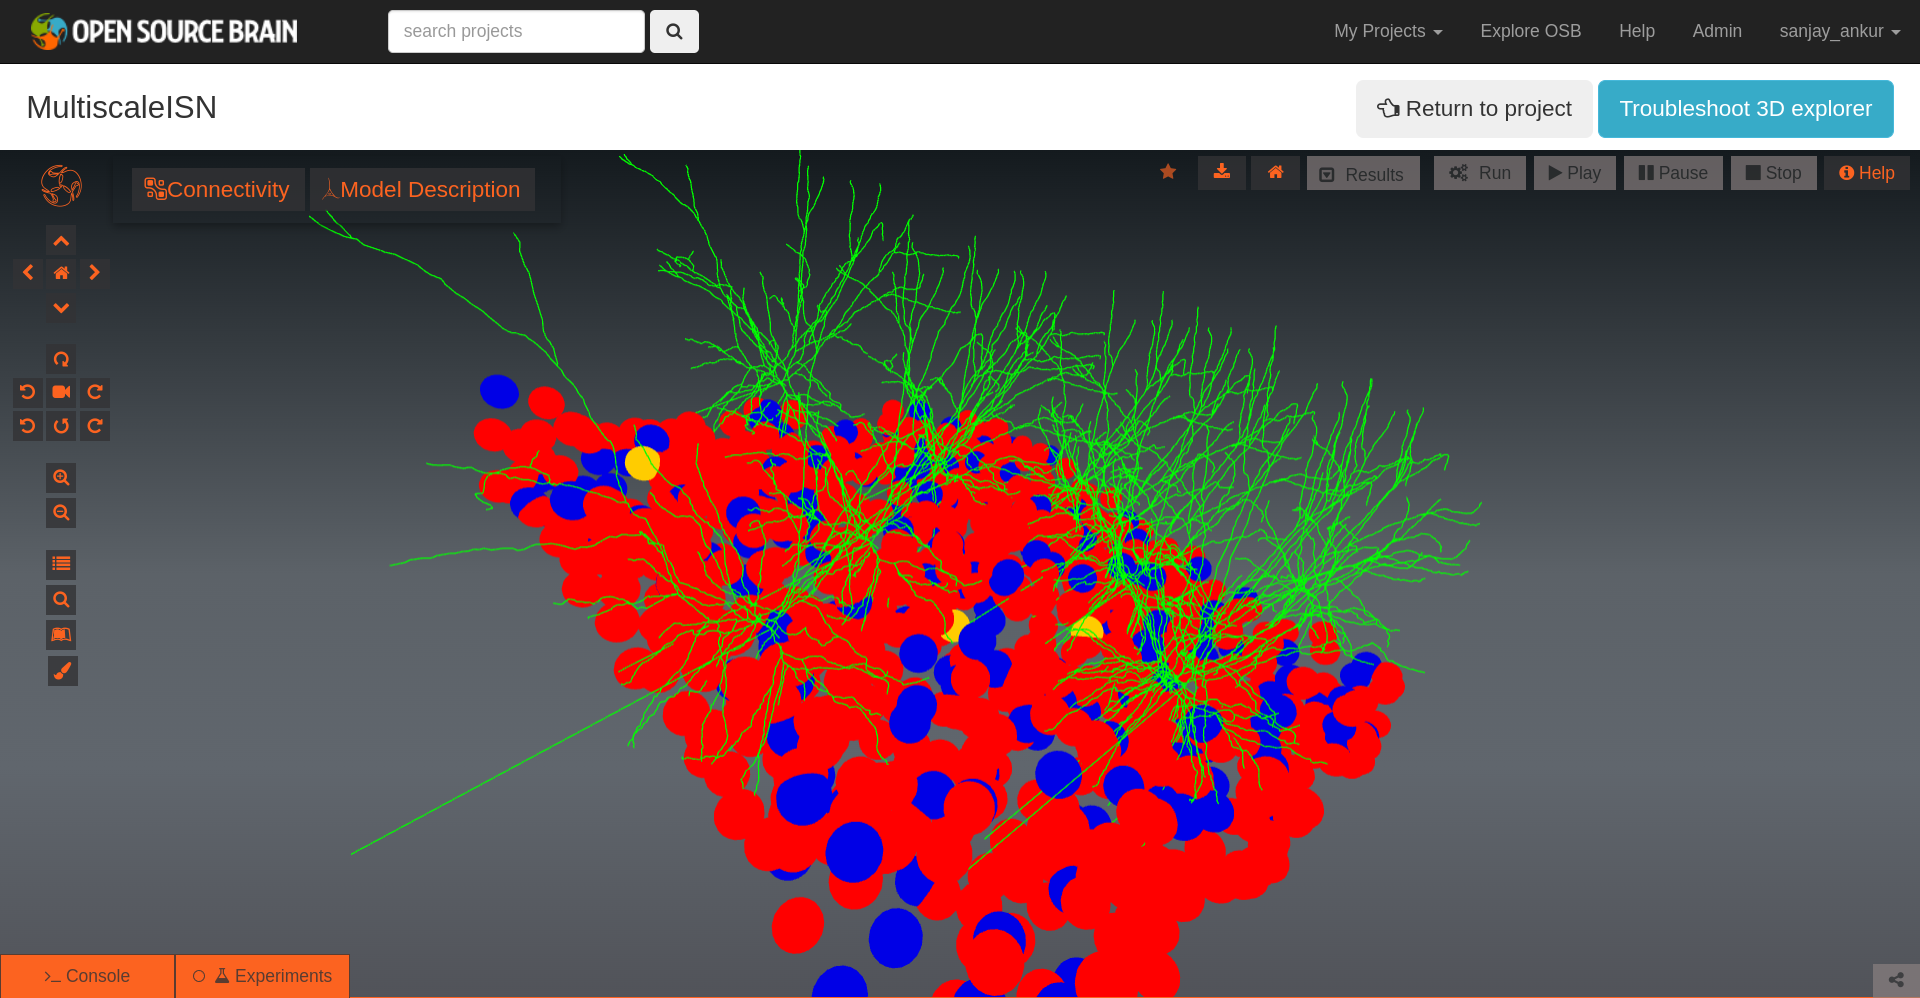
\includegraphics[width=0.9\textwidth]{99_images/20231004-multiscaleisn}}%
    \only<3>{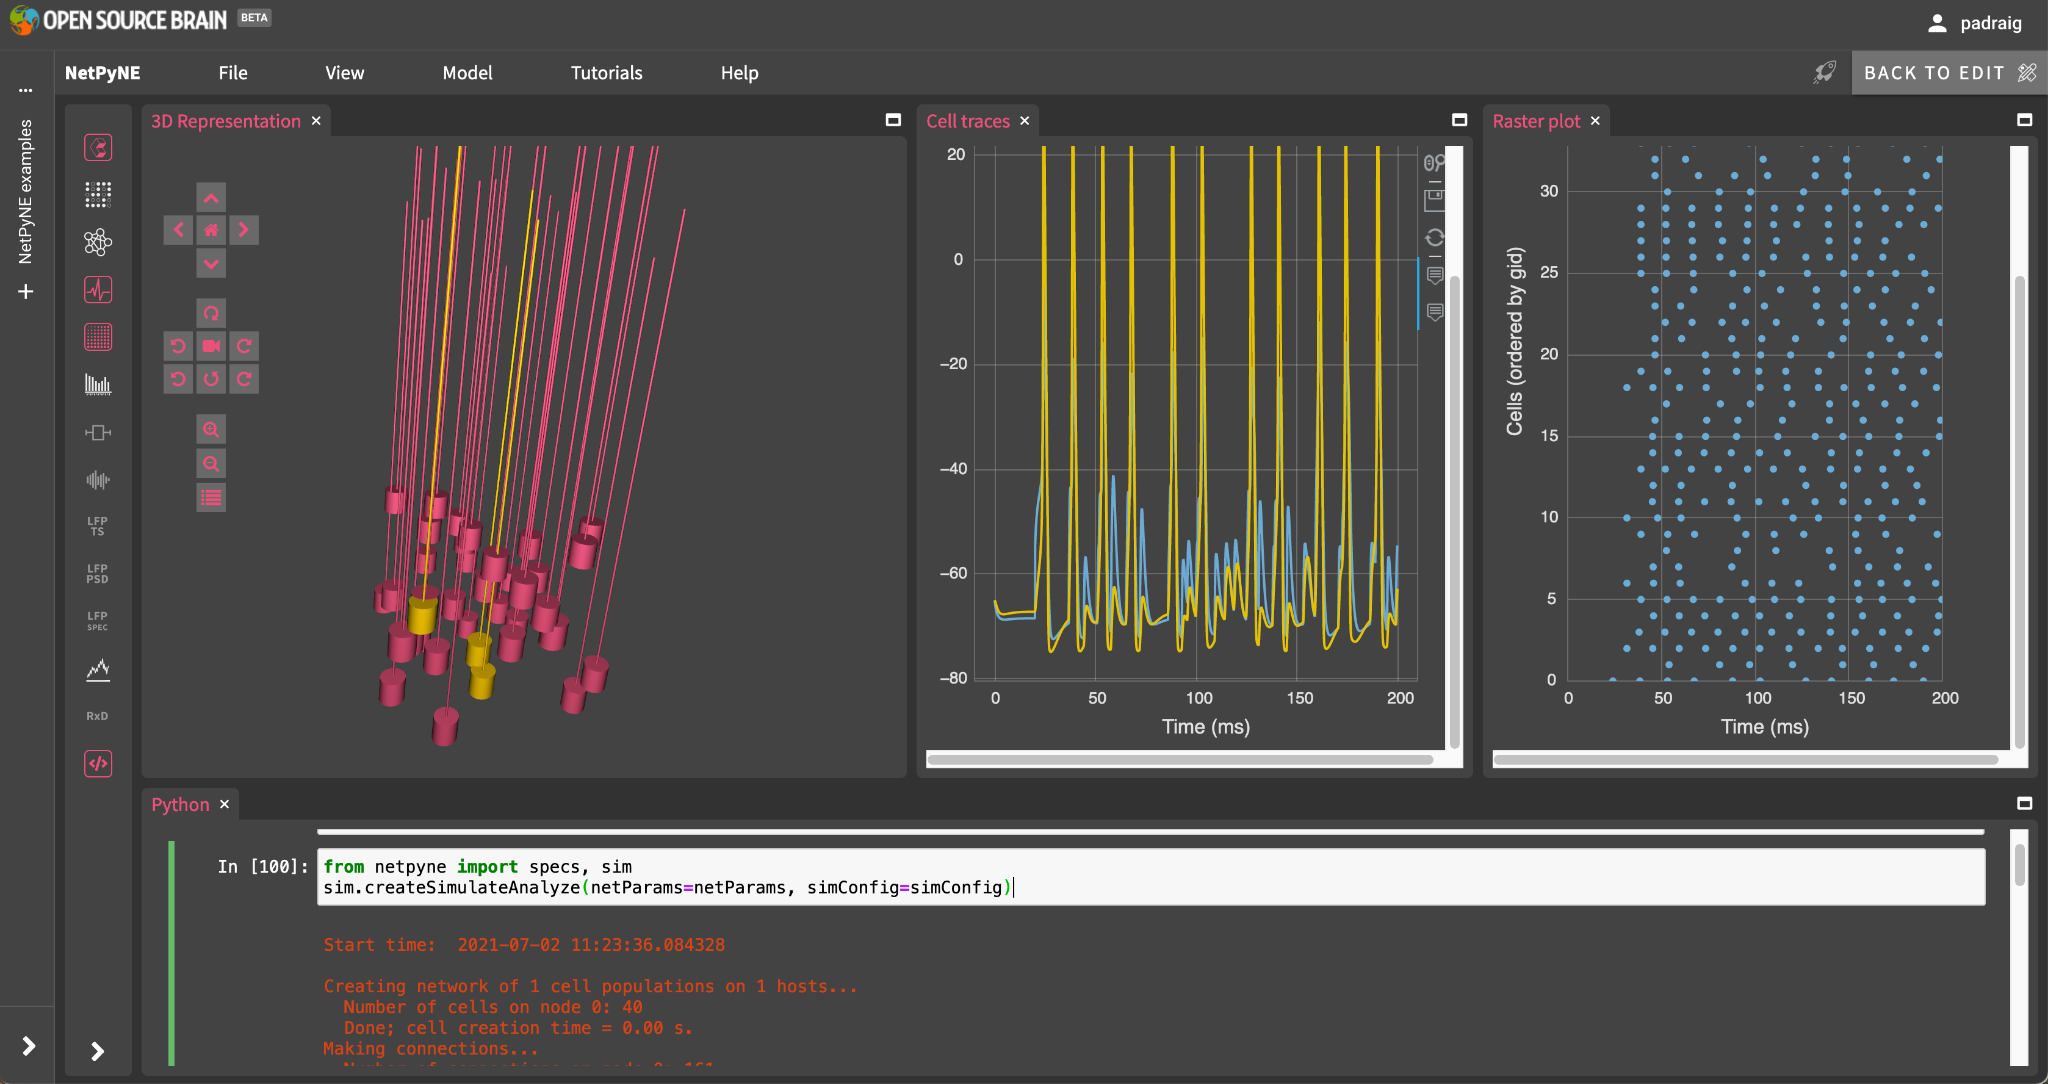
\includegraphics[width=0.9\textwidth]{99_images/20231004-netpyneui}}%
    \only<4>{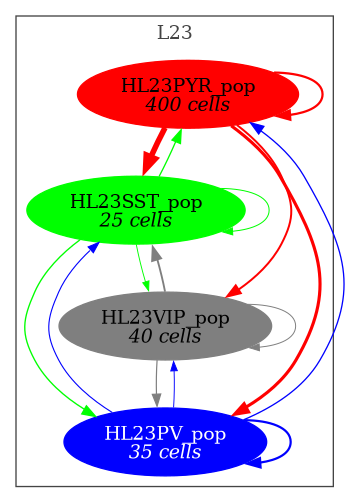
\includegraphics[width=0.31\textwidth,keepaspectratio]{99_images/HL23Network.gv}~~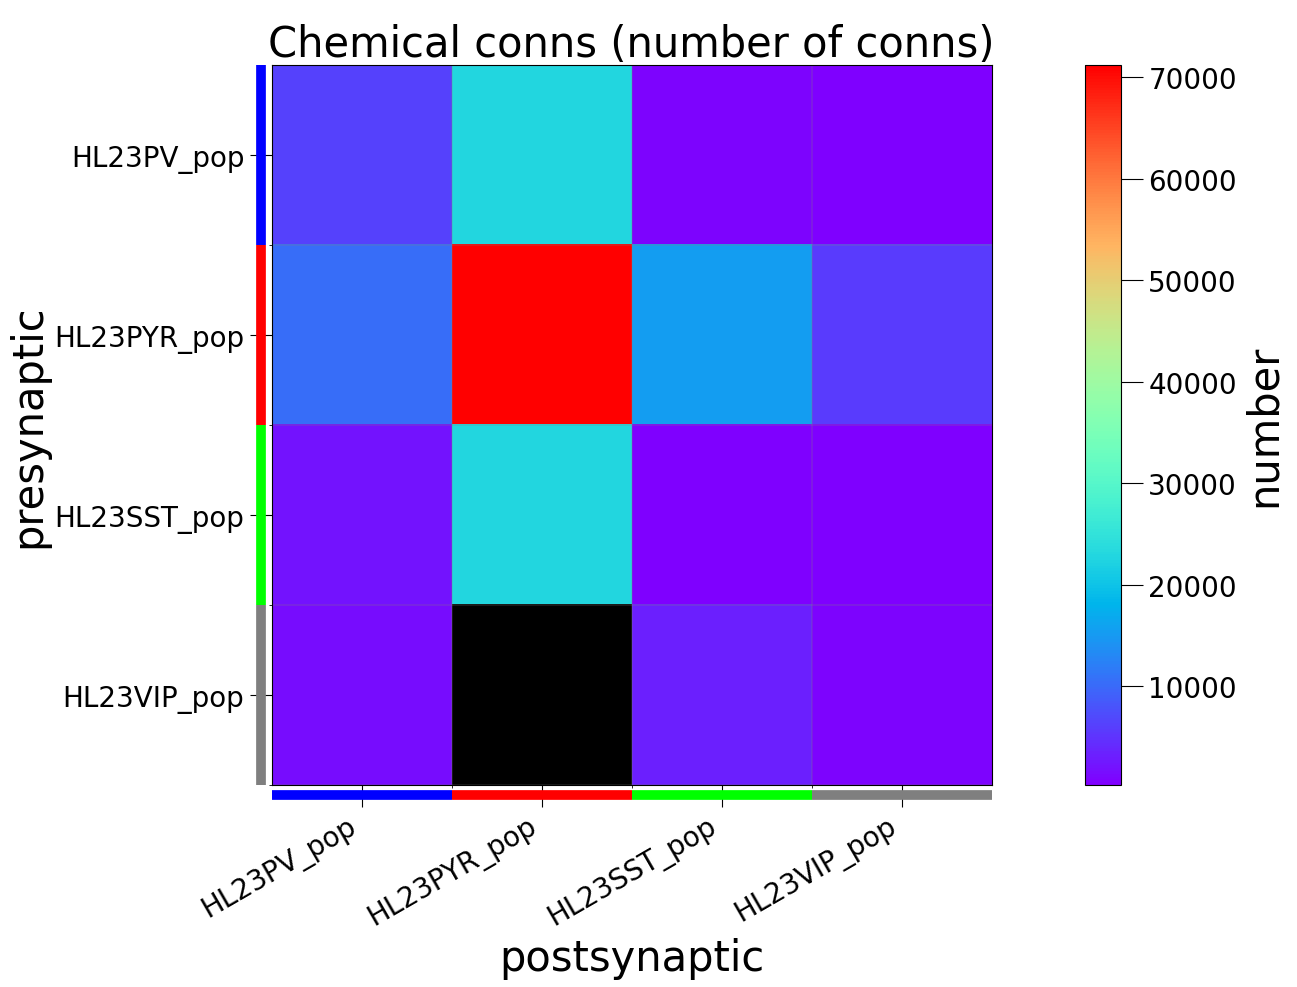
\includegraphics[width=0.6\textwidth,keepaspectratio]{99_images/HL23-con-matrix}}
    \only<5>{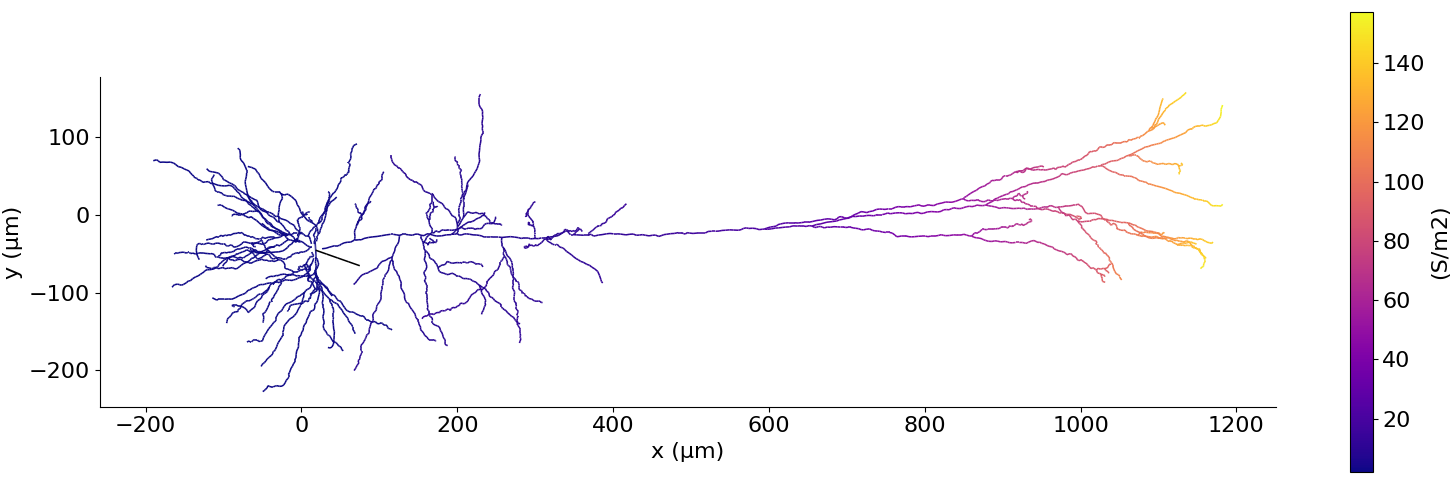
\includegraphics[width=0.9\textwidth,keepaspectratio]{99_images/Ih}}
  \end{figure}
  \only<1>{\footnotetext[1]{3D interactive visualisation of \textcite{Migliore2003} using \texttt{pynml-plotmorph}}}
  \only<2>{\footnotetext[1]{3D interactive visualisation of \textcite{Sadeh2017} on Open Source Brain: \url{https://v1.opensourcebrain.org}}}
  \only<3>{\footnotetext[1]{3D interactive visualisation using NetPyNE-UI on Open Source Brain v2: \url{https://opensourcebrain.org}}}
  \only<4>{\footnotetext[1]{Connectivity metrics for NeuroML conversion of \textcite{Yao2022}}}
  \only<5>{\footnotetext[1]{Automated visualisation of ionic conductance density on a multi-compartmental cell}}
\end{frame}
\begin{frame}[c]
  \frametitle{NeuroML: fitting models}
  \begin{figure}[h]
    \only<1>{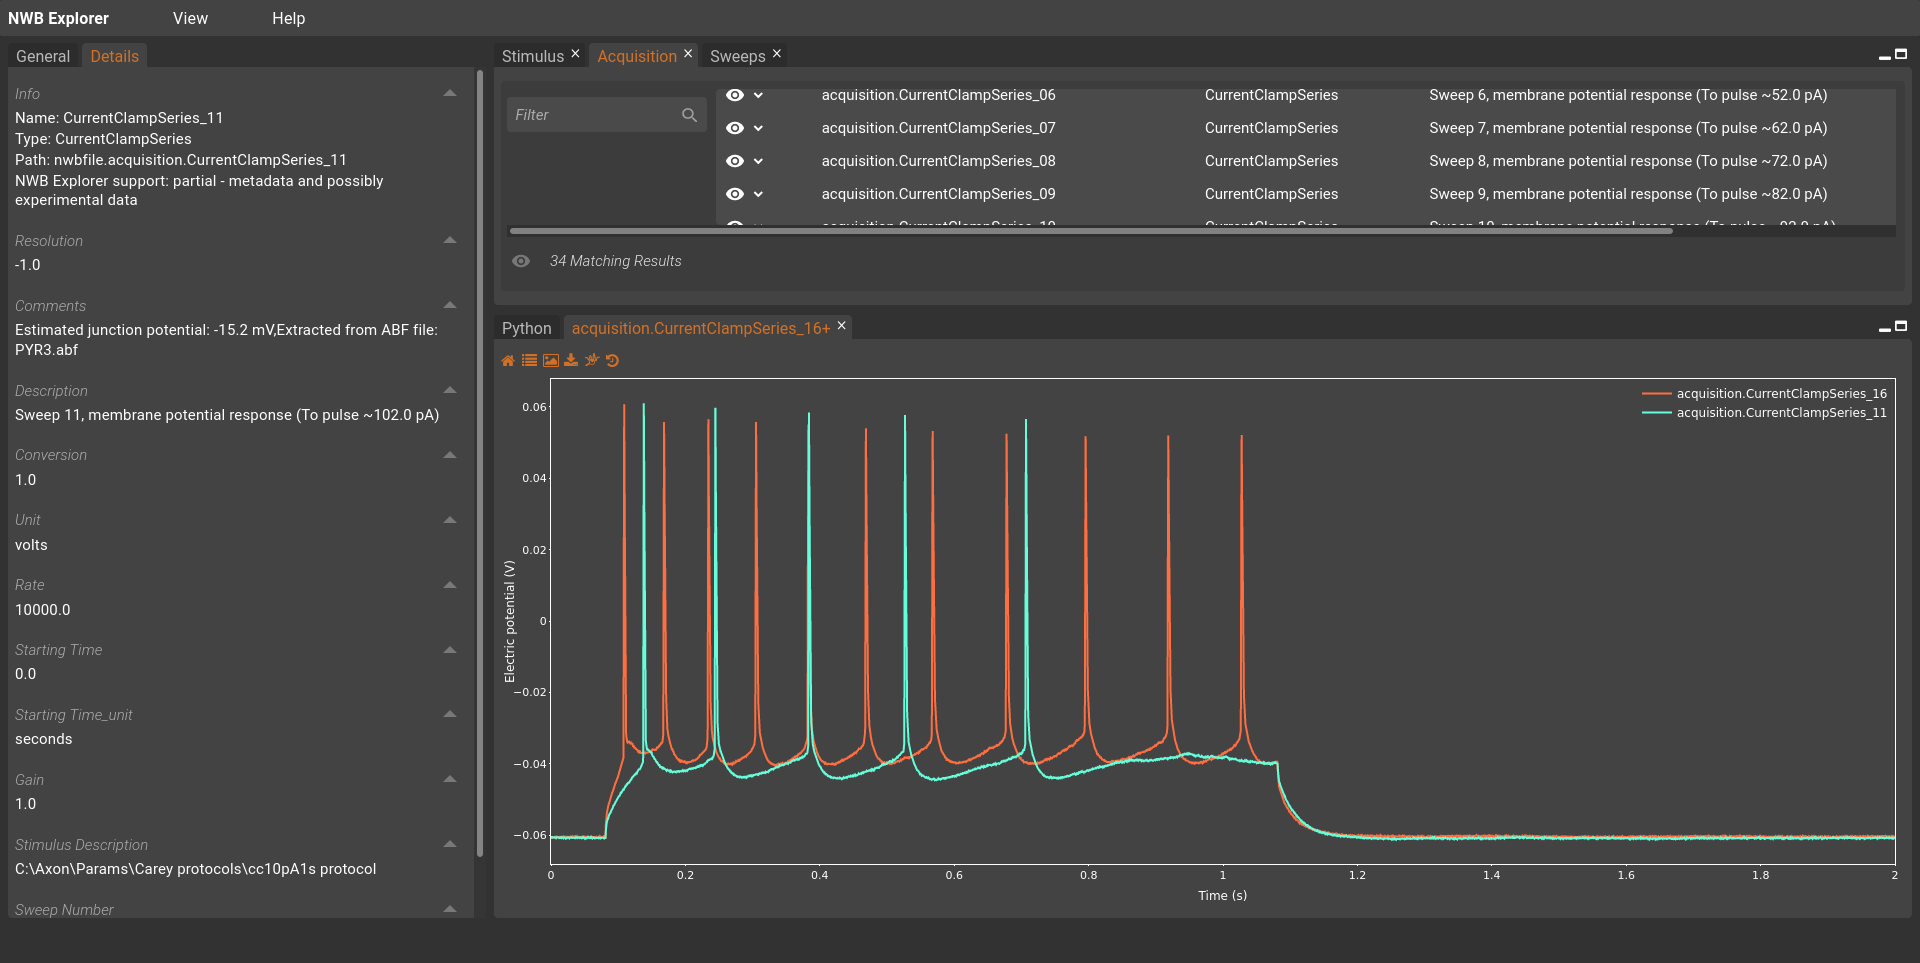
\includegraphics[width=0.9\textwidth]{99_images/fitted_izhikevich_screenshot_nwbexplorer}}%
    \only<2>{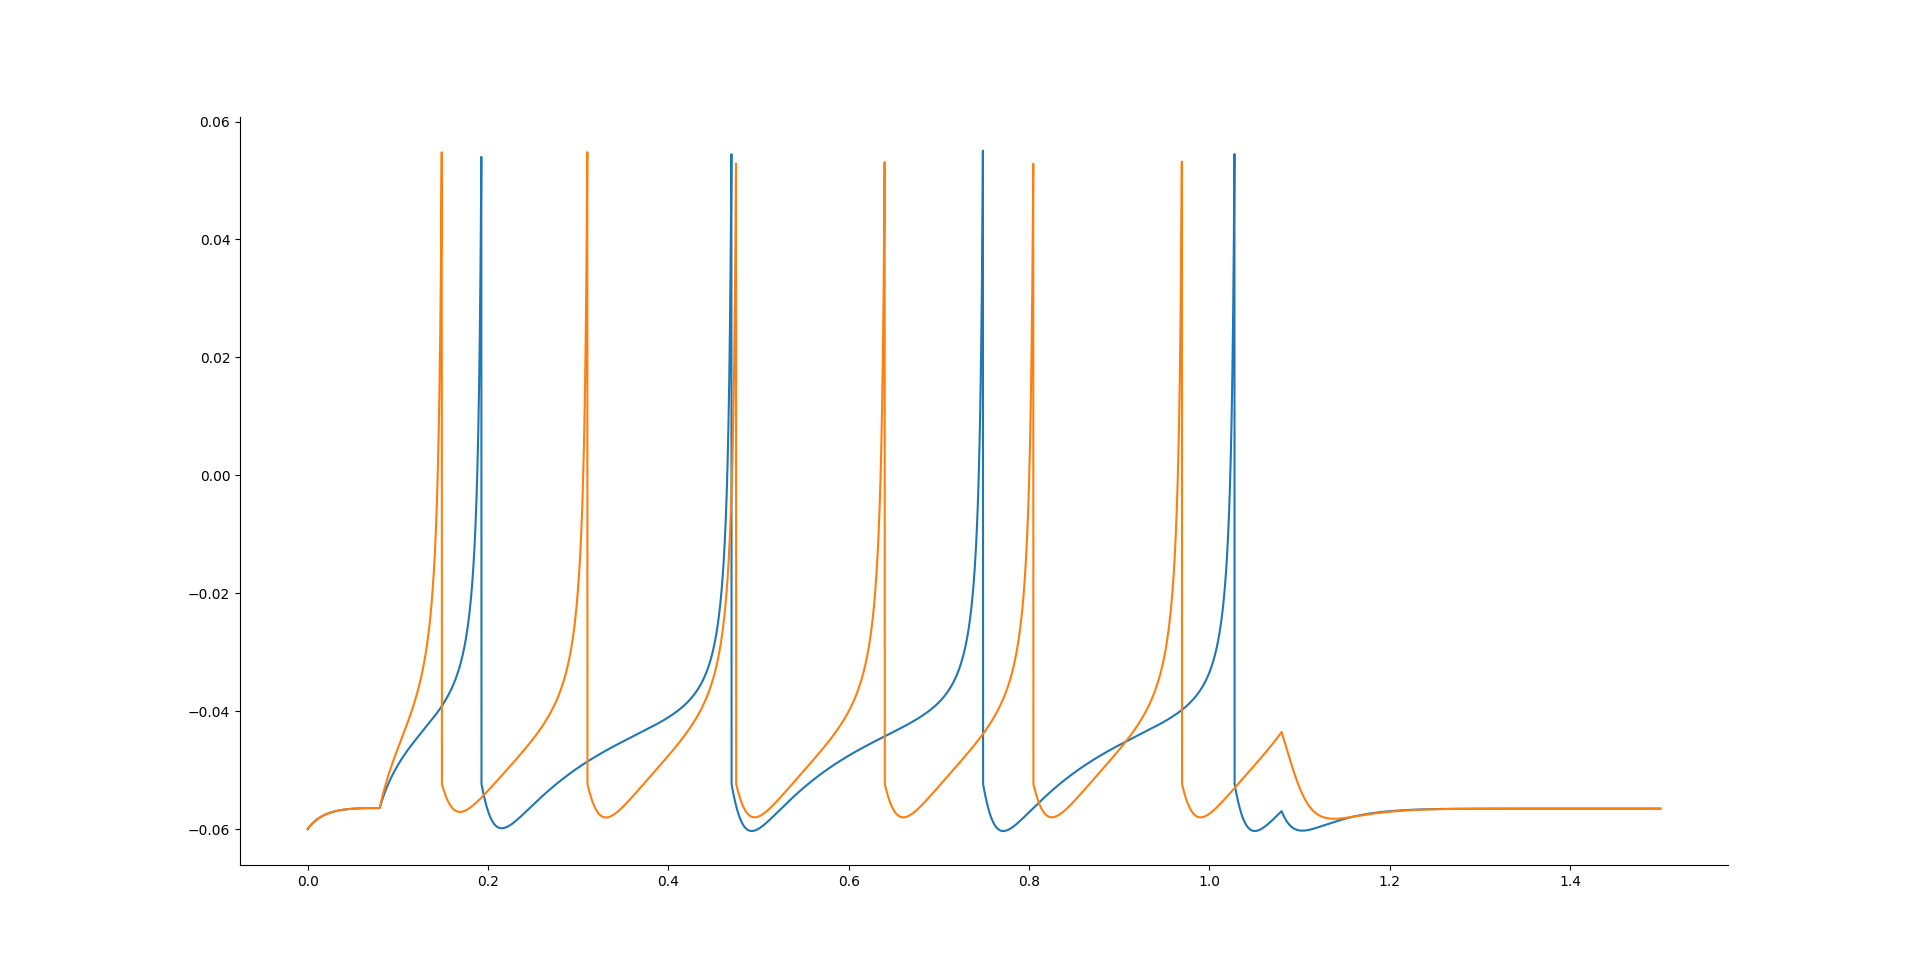
\includegraphics[width=0.9\textwidth]{99_images/izhikevich-fitted-sim}}%
  \end{figure}
  \only<1>{\footnotetext[1]{Visualising \textcite{Lanore2019} in NWB Explorer on Open Source Brain}}
  \only<2>{\footnotetext[1]{Izhikevich cells fitted using NeuroML fitting pipeline: NeuroTune, using Inspyred}}
\end{frame}
\begin{frame}[c]
  \frametitle{NeuroML: sharing and re-using models}
  \begin{figure}[h]
    \only<1>{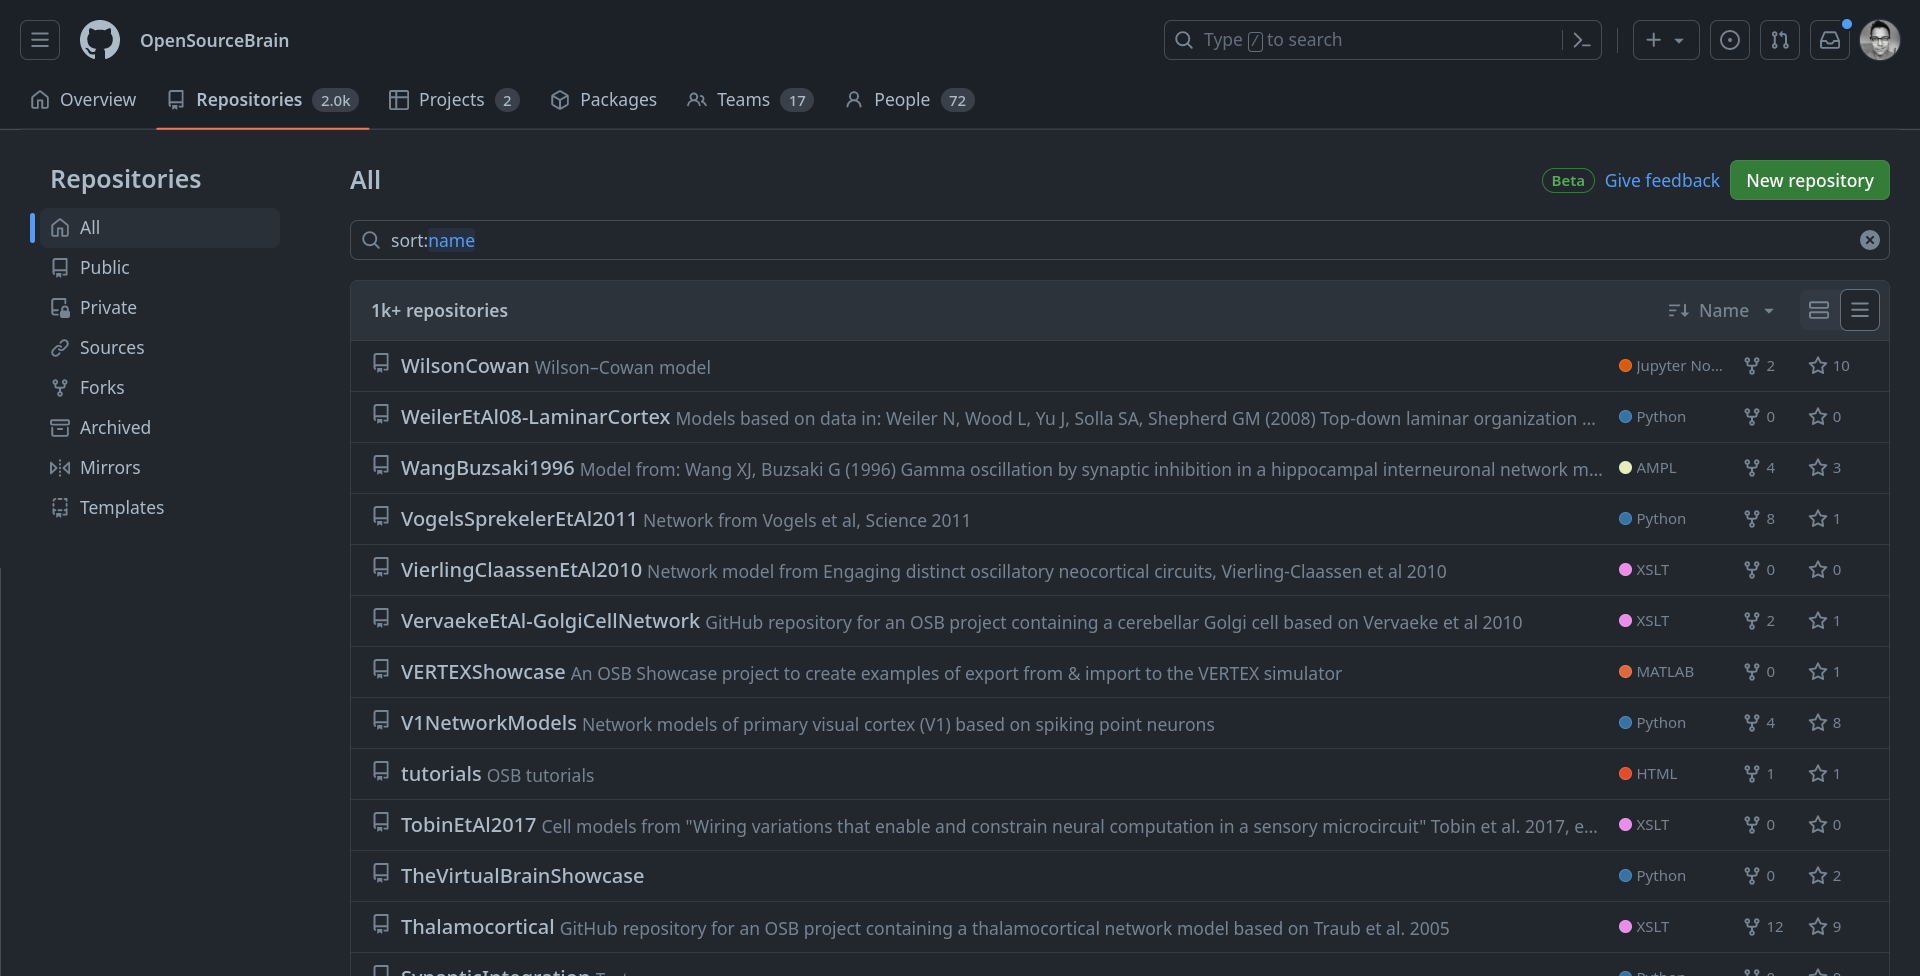
\includegraphics[width=0.9\textwidth]{99_images/osb-repolist}}%
    \only<2>{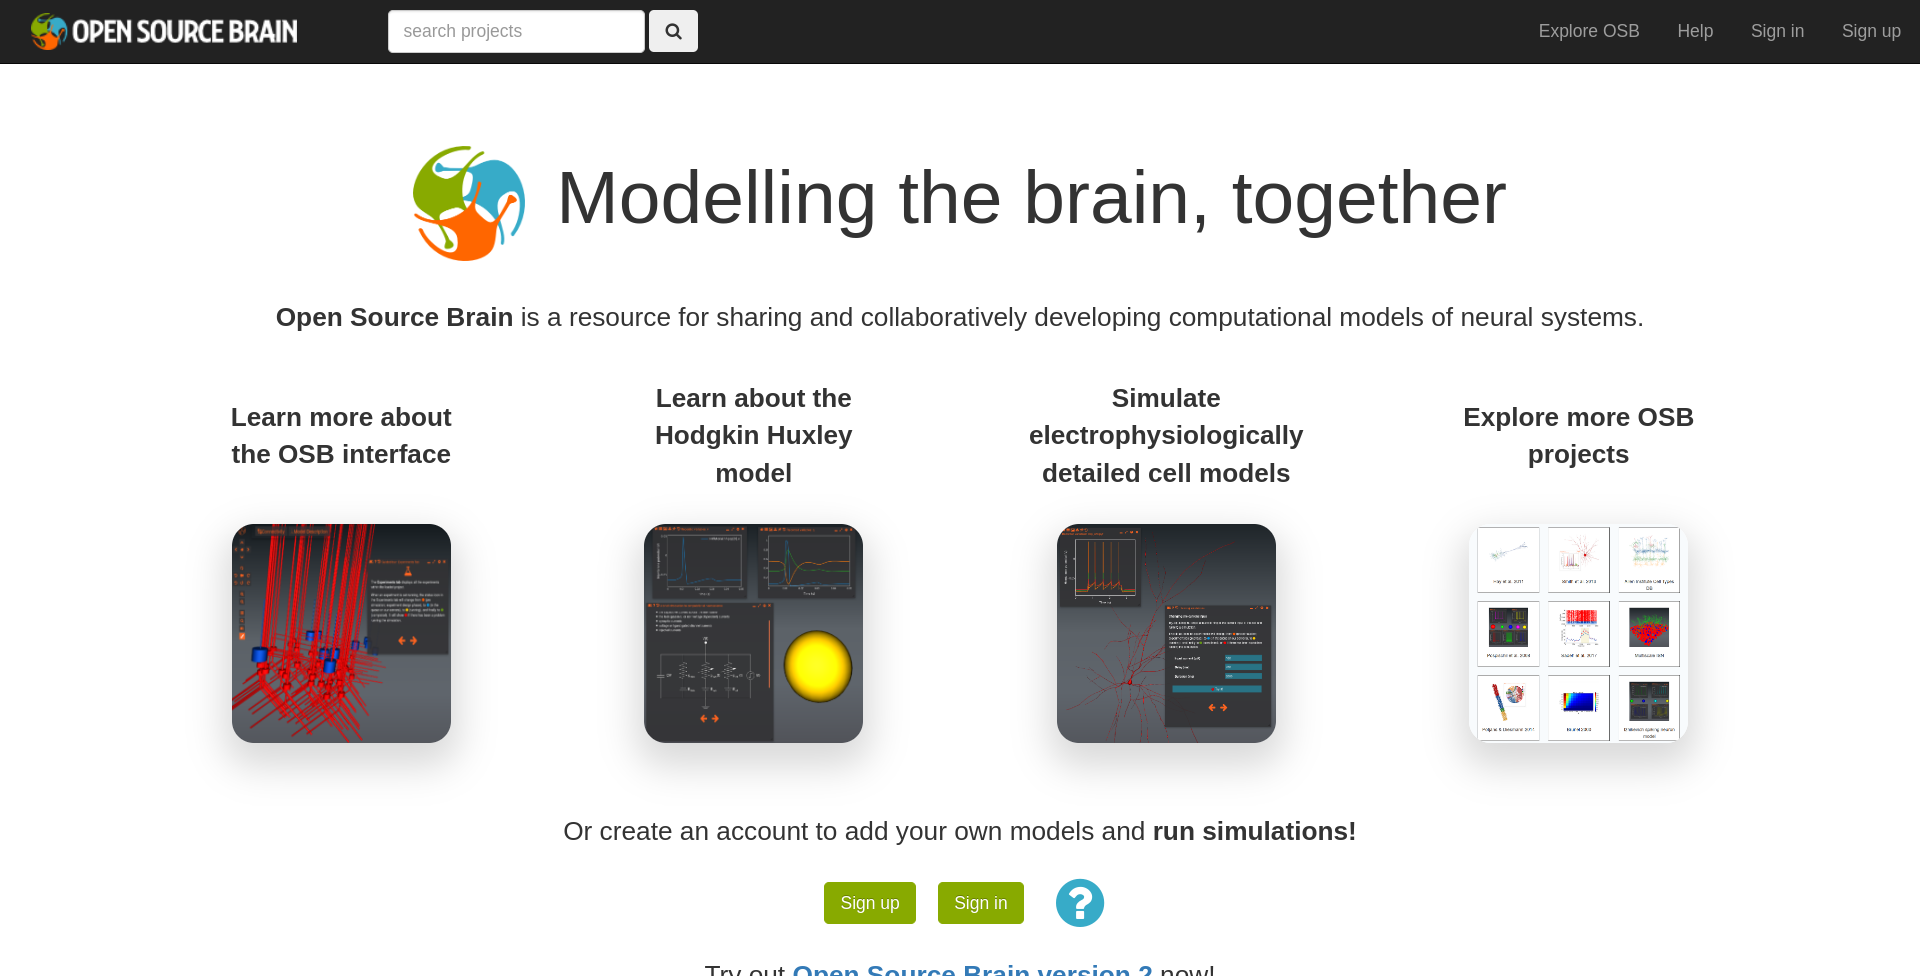
\includegraphics[width=0.9\textwidth]{99_images/osbv1}}%
    \only<3>{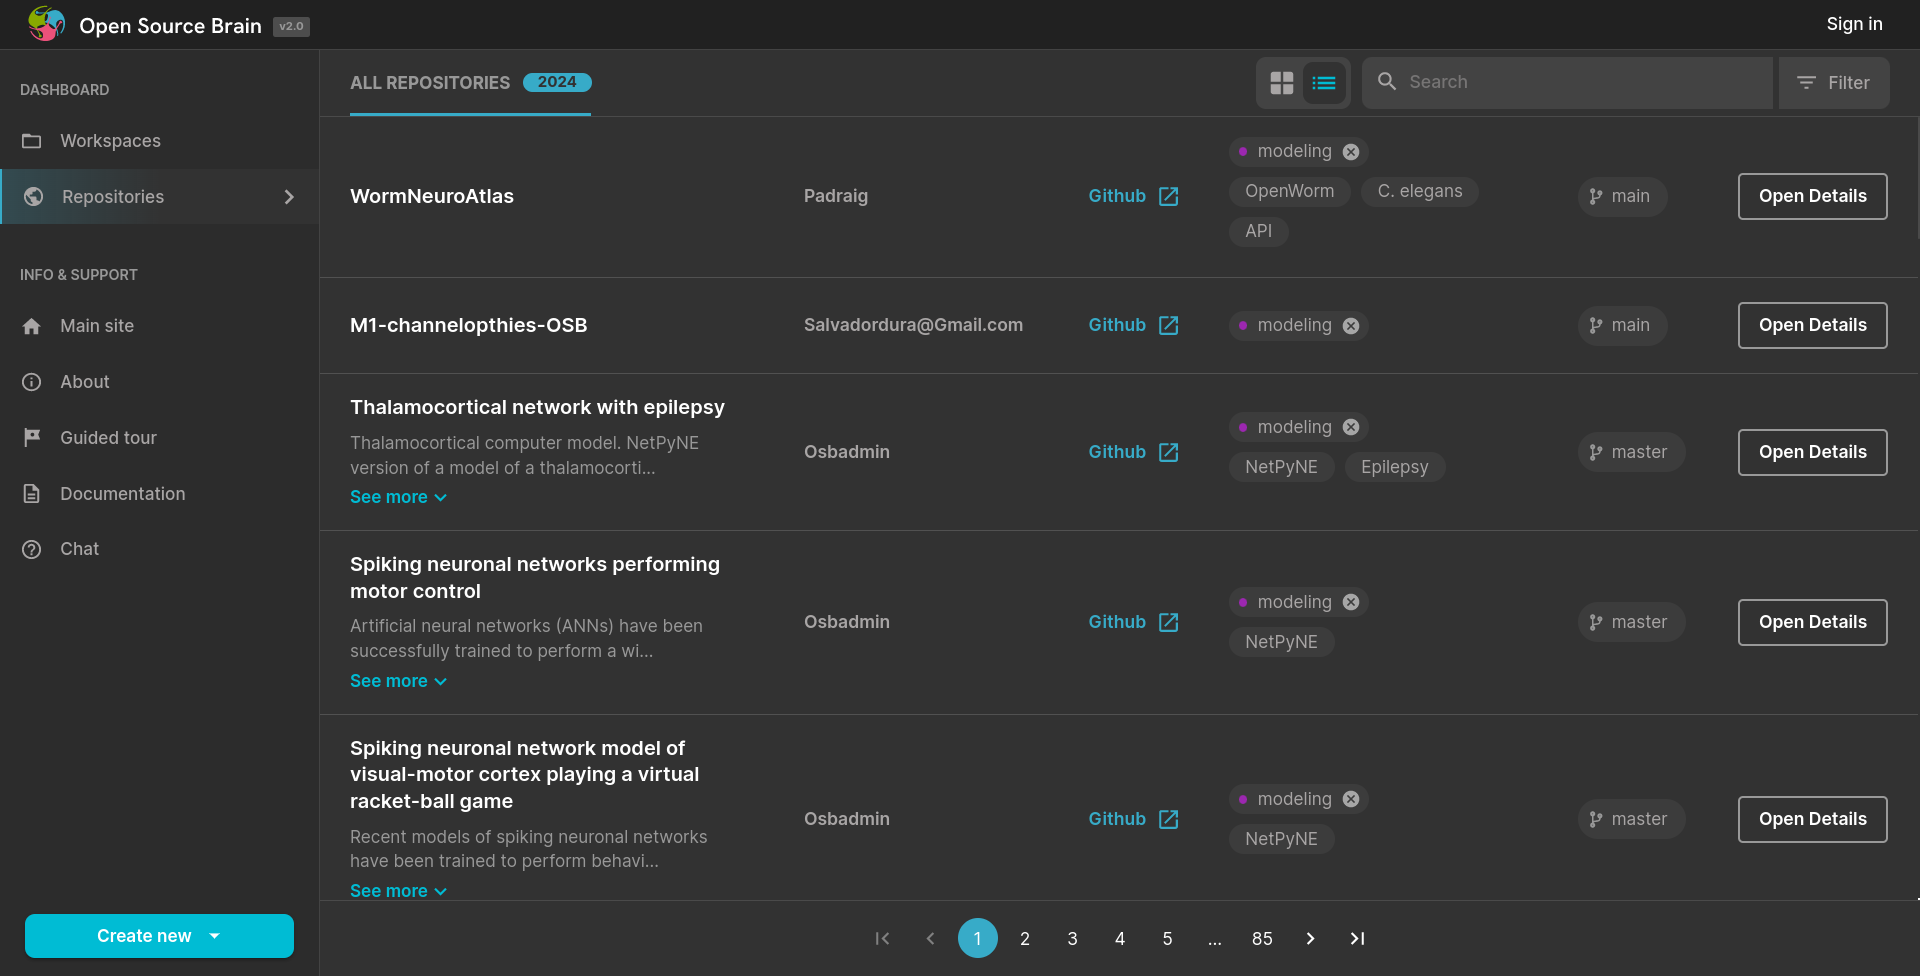
\includegraphics[width=0.9\textwidth]{99_images/osbv2}}%
    \only<4>{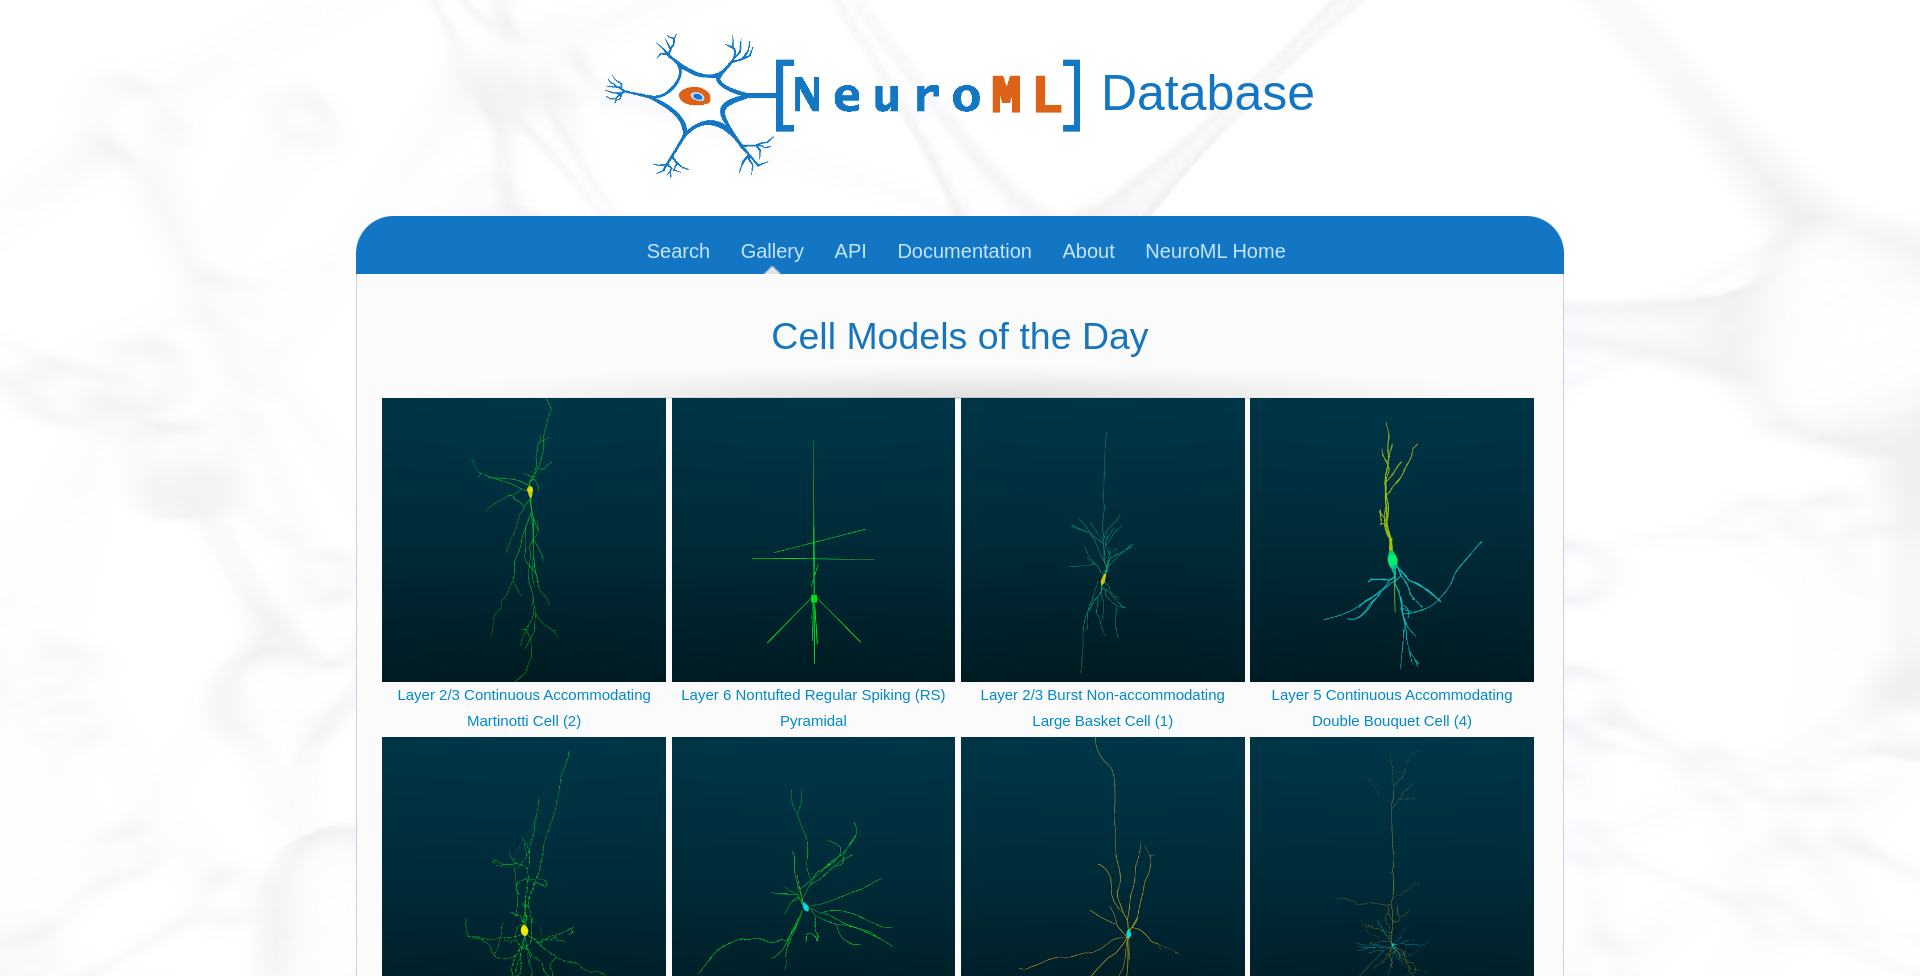
\includegraphics[width=0.9\textwidth]{99_images/neuromldb}}%
  \end{figure}
  \only<1>{\footnotetext[1]{Standardized models on Github: Open Source Brain: \url{https://github.com/OpenSourceBrain}}}
  \only<2>{\footnotetext[1]{Standardized models on Open Source Brain v1: \url{https://v1.opensourcebrain.org}}}
  \only<3>{\footnotetext[1]{Standardized models on Open Source Brain v2: \url{https://v2.opensourcebrain.org}}}
  \only<4>{\footnotetext[1]{Standardized models on NeuroML-DB: \url{https://neuroml-db.org}}}
\end{frame}
%\section{Under the hood}
\begin{frame}[c]
  \frametitle{NeuroML: community: events}
  \begin{figure}[h]
    \only<1>{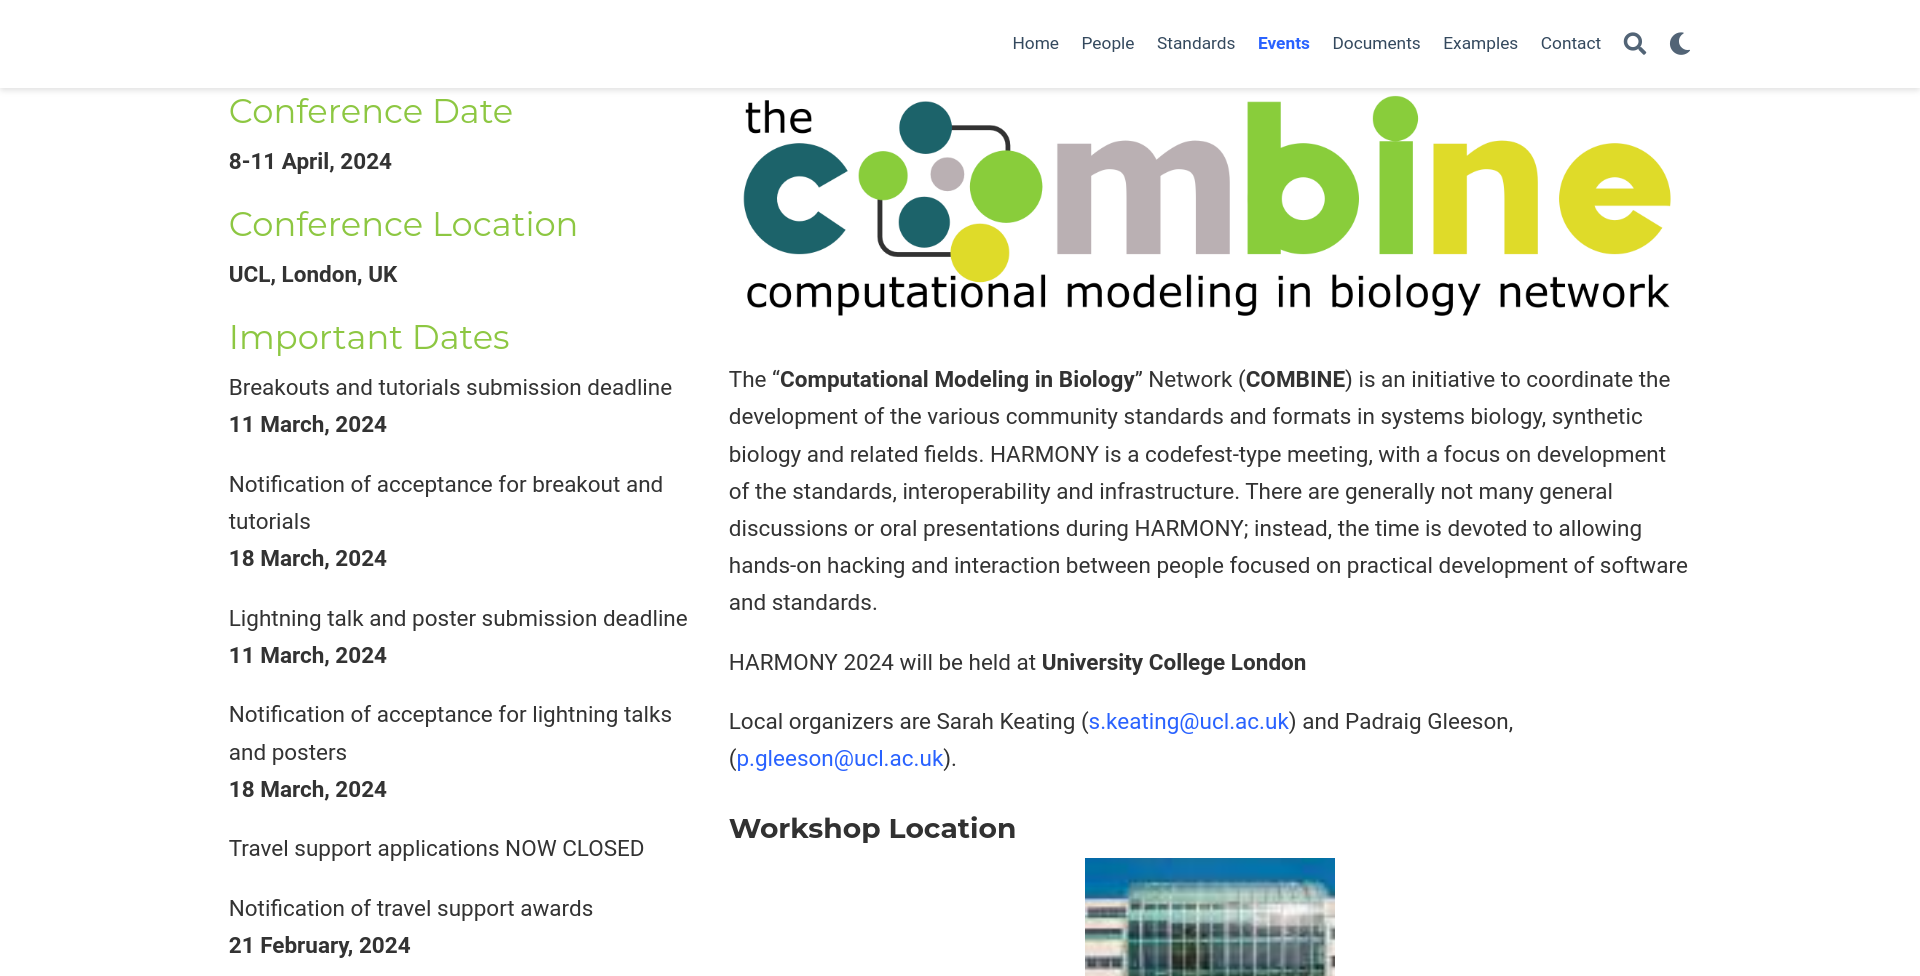
\includegraphics[width=0.9\textwidth]{99_images/harmony2024}}%
    \only<2>{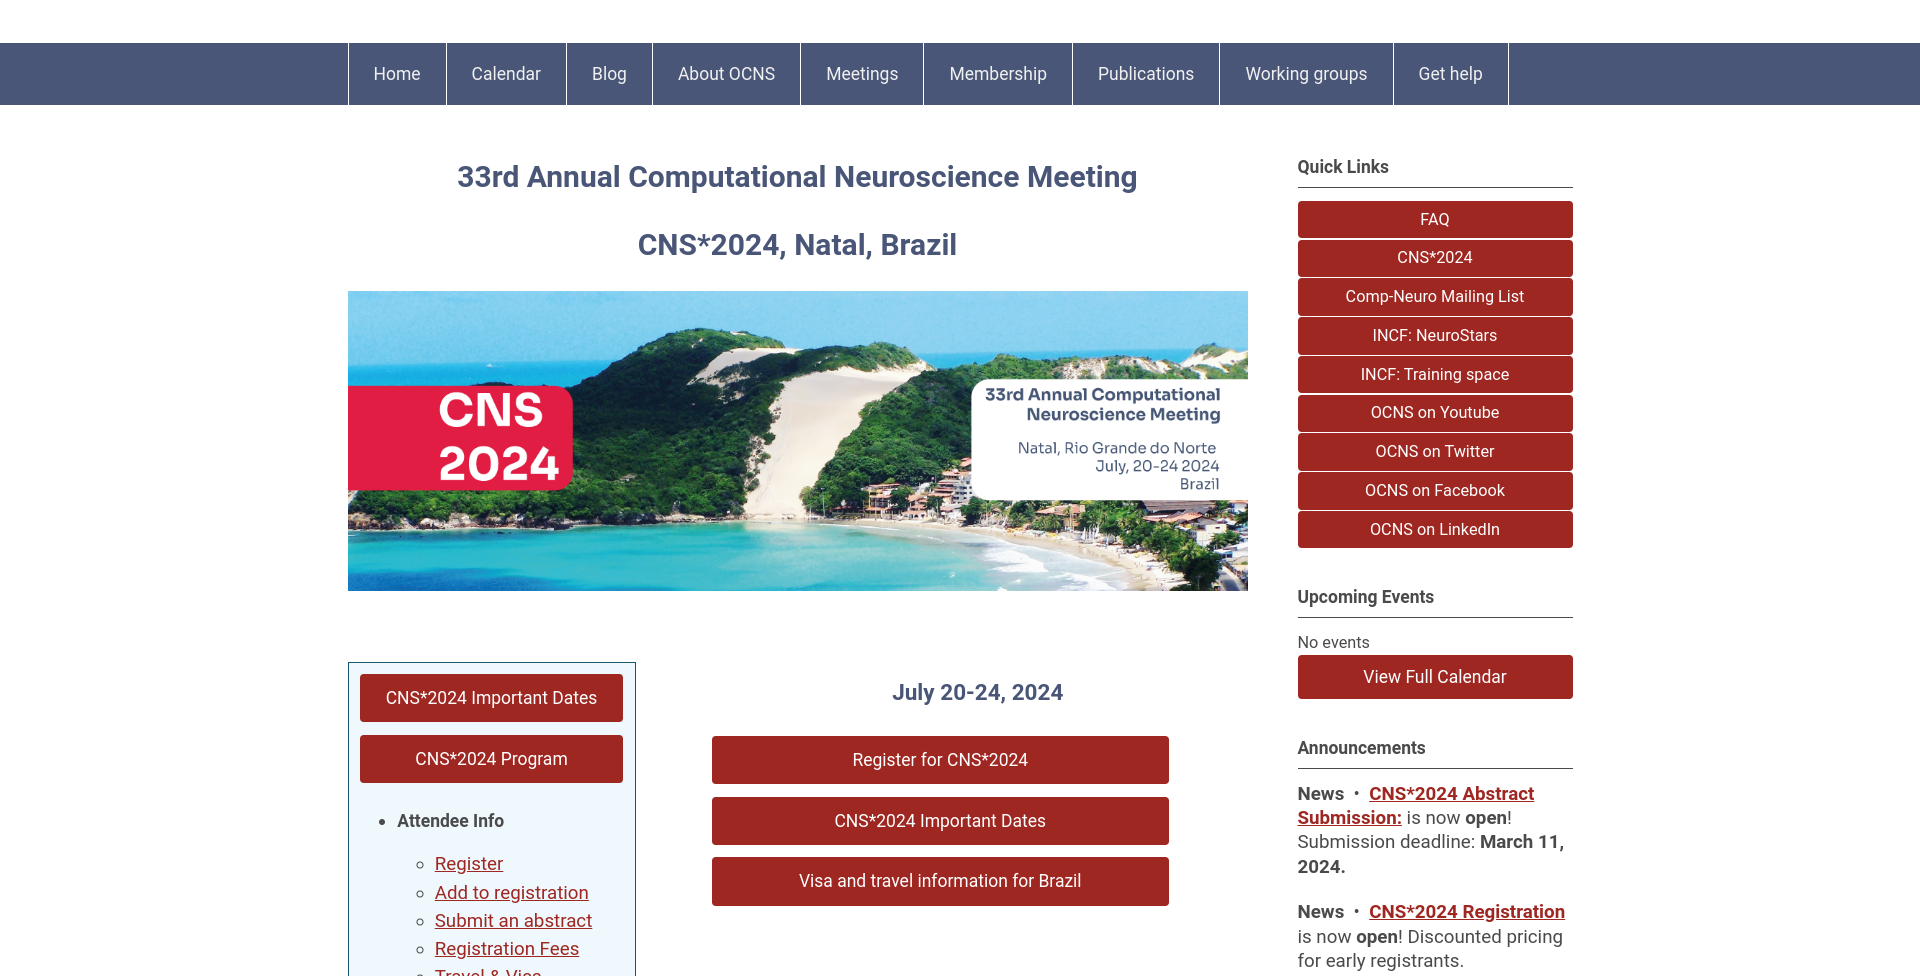
\includegraphics[width=0.9\textwidth]{99_images/cns2024}}%
  \end{figure}
  \only<1>{\footnotetext[1]{\url{https://co.mbine.org/events/}}}
  \only<2>{\footnotetext[1]{\url{https://www.cnsorg.org}}}
\end{frame}
\begin{frame}[c]
  \frametitle{NeuroML: projects: GSoC}
  \begin{itemize}
    \item Open source, cross simulator, large scale network models in NeuroML and PyNN.
    \item Implementation of SWC to NeuroML converter in PyNeuroML
    \item Incorporate new features into an advanced, cross-platform 3D viewer for NeuroML cells and networks
  \end{itemize}
\end{frame}
\begin{frame}[c]
  \frametitle{NeuroML: closing the neuroscience research loop with OSB}
  \begin{itemize}
    \item Open Source Brain Video
  \end{itemize}
\end{frame}
% last slide
\begin{frame}[c]
  \frametitle{NeuroML: resources}
  \begin{center}
    \fullcite{Sinha2023}(in review)\\\vspace{1cm}
    \Large{\url{https://docs.neuroml.org}}\\
    \Large{\url{https://opensourcebrain.org}}
  \end{center}
\end{frame}
\end{document}
